% Document class / Dokumentenklasse:
\documentclass{LNTthesis}
% Parameters of the LNTthesis class:
% DIV12       = document layout: DIV factor = 12 (larger number creates larger pages)
% BCOR12mm    = binding correction: 12mm
% headsepline = separate page head by a line
% twoside     = twosided document
% 11pt        = font size 11 point
% openright   = start new chapters only on right pages (odd numbered pages)
% more information: http://tug.ctan.org/tex-archive/macros/latex/contrib/koma-script/scrguien.pdf

% Packages used in LNTthesis class:
% package[english]{babel}   % english language / Englische Sprache
% package{LNTthesis}        % LNT specific definitions / LNT spezifische Definitionen
% package{graphicx}         % for using eps images / Einbinden von EPS Grafiken
% package{verbatim}         % for quickly commenting out large parts of your text / Um viel Text schnell auskommentieren zu koennen
% package{amssymb}          % additional math symbols / Zusaetzliche mathematische Symbole
% package{amsmath}          % additional math commands / Zusaetzliche mathematische Befehle
% package{amsxtra}          % even more math symbols / Noch mehr mathematische Symbole
% package{amsthm}           % theorem environment etc / Theorem Umgebung usw
% more information on amsmath: http://www.ctan.org/get/macros/latex/required/amslatex/math/amsldoc.pdf

% package{psfrag}           % psfrag: http://www.ctan.org/get/macros/latex/contrib/psfrag/pfgguide.pdf
% package{subfigure}        % enable subfigures / Ermoeglicht Subfigures (mehrere Figures neben/untereinander)

% !! PLEASE READ THE LATEX HELP IF YOU HAVE ANY QUESTIONS !!
% http://tobi.oetiker.ch/lshort/lshort.pdf


% Macros:
    \newcommand{\eq}[1]{Equation (\ref{#1})}        % \eg{eq:golomb}  --> Equation (2.15)
    \newcommand{\eref}[1]{(\ref{#1})}               % \eg{eq:golomb}  --> (2.15)
    \newcommand{\fig}[1]{Figure \ref{#1}}           % \fig{fig:golomb}--> Figure 2.15
    \newcommand{\tab}[1]{Table \ref{#1}}            % \tab{tab:lala}  --> Table 2.15
    \newtheorem{prop}{Proposition}

% Abbreviations
    \newcommand{\equivalent}{\triangleq}
    \newcommand{\given}{\:\!\vert\:\!}


% ########################################
% Yadhu defined
% #########################################
\newcommand\TODO[1]{\textcolor{red}{#1}}

\newcommand\NOTE[1]{\textcolor{blue}{#1}}

\DeclarePairedDelimiter\ceil{\lceil}{\rceil}
\DeclarePairedDelimiter\floor{\lfloor}{\rfloor}

\newenvironment{code}{\captionsetup{type=listing}}{}
\SetupFloatingEnvironment{listing}{name=\textbf{Listing}}


% Document:
\begin{document}

% ###################################
% Title page / Titelseite
% ###################################
\LNTtitle{Master's Thesis}          % Thesis type / Art der Arbeit (Master's Thesis, Diplomarbeit)
    {Polar FEC chain development in software for 5G}                  % Thesis title / Titel der Arbeit
    {Yadhunandana Rajathadripura Kumaraiah}                  % Your name / Name des Diplomanden
    {Dr. Moritz Harteneck, Alexander Heinz, Rohde \& Schwarz \newline
 	 Fabian Steiner M.Sc,
 	 Peihong Yuan M.Sc}                % Advisor / Betreuer
    {M\"unchen, November 2018}          % Munich, Date / Muenchen, Datum
    {Yadhunandana Rajathadripura Kumaraiah\\                 % Your Address / Anschrift des Diplomanden
    Schr\"ofelhofstra\ss e 14 WG 02/02\\
    81375 M\"unchen\\
    yadhu.kumaraiah@tum.de}

\LNTrecht{Yadhunandana Rajathadripura Kumaraiah}             % Your name / Name des Studenten
    {M\"unchen, 12.09.2018}         % Munich, Date / Muenchen, Datum

\cleardoubleemptypage   % start new double page / neue Doppelseite

% ########################################
% Table of Contents / Inhaltsverzeichnis
% ########################################

% roman page numbering, starting with page number 1 / roemische Seitennummerierung beginnend mit Seite 1
    \setcounter{page}{1}
    \pagenumbering{roman}

        \tableofcontents    % Table of contents / Inhaltsverzeichnis
        \listoffigures      % List of figures / Abbildungsverzeichnis
        \listoftables       % List of tables / Tabellenverzeichnis
        \cleardoubleemptypage   % start new double page / neue Doppelseite

% ########################################
% Chapters / Kapitel:
% ########################################

% arabic page numbering, starting with page number 1 / arabische Seitennummerierung beginnend mit Seite 1
    \setcounter{page}{1}
    \pagenumbering{arabic}

        %%%%%%%%%%%%%%%%%%%
\chapter*{Abstract}
%%%%%%%%%%%%%%%%%%%
Software implementation of error correction and signal processing applications on general purpose processors has gained interest in recent times. Mainly due to latest technological developments in general purpose computing world. Implementations in software have an inherent advantage not being tied to one specific hardware architecture. They require much less development and maintenance effort compared hardware implementations. For the device manufacturer software implementation provides platform flexibility in addition to reducing the cost of product. \newline

In this thesis, we study the feasibility of developing complete polar FEC chain of $5^{th}$ generation cellular mobile communication standard in software. Specifically on general purpose processors. Thesis work attempts to achieve stringent latency requirements through software, algorithmic and platform specific optimizations. Many algorithms in FEC chain are optimized for hardware implementations. Direct implementation of these algorithms in software results in poor performance. To obtain best performance on general purpose processors these algorithms are modified or reformulated to suit software implementation. Initially both encoding and decoding FEC chain are implemented functionally without any algorithm reformulation or optimization. Code profiling is performed on this naive implementation to identify the significant latency contributors. We split algorithms of significant latency contributing components into primitive operations. These primitive operations are mapped to specialized functional units of general purpose processor to achieve best performance. \newline

We concentrate on polar encoding and decoding FEC chain which are used transmitting control information. Latency contributing components are identified. Algorithms of those components are reformulated to avoid or to reduce latency contributing operations. Major latency contributors in encoding FEC chain were Cyclic redundancy check (CRC) calculation, polar code construction, polar encoding. In decoding FEC chain  subblock deinterleaver, polar decoder, parity bit extraction, CRC calculation. Algorithms of these components are reformulated to suit software requirements and implemented using efficient \emph{vector processing instruction sets}. Algorithms are modified to reduce complexity and lookup tables are used to avoid complex computations. Other optimizations include function unrolling, avoiding superfluous copy operations, hints to compiler for better instruction scheduling and block wise copying et cetera. At the end of both encoding and decoding chapter latency comparisons between naive and optimization are presented. In decoding FEC chain chapter, latencies of decoder of this work and state of the art decoder are compared.     % Include abstract / Einbinden von Kurzfassung und Abstract
        %%%%%%%%%%%%%%%%%%%%%%%%%%%%%%%%%%%%%%%%%%%%%%%
\chapter{Introduction and Motivation} \label{chap:introduction}
%%%%%%%%%%%%%%%%%%%%%%%%%%%%%%%%%%%%%%%%%%%%%%%



In 1948, scientists at the Bell Laboratories achieved two landmark research results:
Claude E.~Shannon published his paper \emph{A mathematical theory of communication} and John Bardeen, Walter Brattain and William Shockley announced the invention of the \emph{transistor effect}.

\cite{Arikan}

A binomial distribution is shown in Figure~\ref{fig:coin_bino}.

\begin{figure}[!htb]
    \centering
    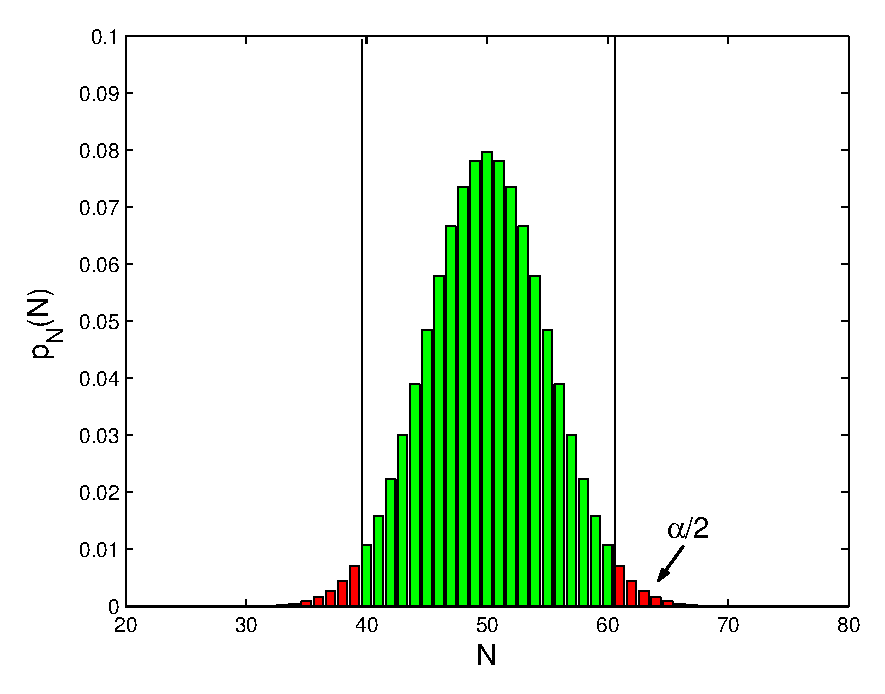
\includegraphics[width=0.8\textwidth]{./figures/coin_bino.eps}
    \caption{PDF $p_N(N)$ of the number N of times that the head side is up.}
    \label{fig:coin_bino}
\end{figure}

For further information, the reader is referred to~\cite{Cover}.\newline

Traditionally FEC chains are developed in hardware i.e FPGA’s or ASIC’s to achieve low latency and high throughput.
Development in FPGA/hardware requires more time and costly.
With recent advances in General Purpose Processors it is possible to achieve required latency and throughput with software implementations without custom hardware.
Software implementations are flexible and easy to maintain compared hardware implementations.

However algorithms need to be adopted/optimized to efficiently implement in software.

Recent advances in the modern processors such as SIMD units can be utilized to achieve low latency and high throughput.



\clearpage
  % Include introduction / Einbinden des Kapitels Einleitung/Problemstellung
        \chapter{Background} \label{chap:Background}

\setcounter{secnumdepth}{3}
\renewcommand{\thesubsubsection}{\Alph{subsubsection}}

%\titleformat{\subsubsection}
%{\selectfont}{\thesubsubsection}{1em}{}

%Give background about polar codes and their adoption in 5G.

Polar codes were introduced by Arikan in his seminal work \cite{Arikan}. They belong to the class of capacity achieving codes. In the past decade, polar codes have sparked a interest from both academia and industry alike, resulting in significant research work in improving performance. The 5\textsuperscript{th} generation wireless systems (5G) standardization has adopted polar codes for uplink and downlink control information for the enhanced mobile broadband (eMBB). They are also considered as the potential coding schemes for two other frameworks of 5G, namely ultra-reliable-low-latency (URLLC) and massive machine-type communications (mMTC).

Polar codes achieve capacity asymptotically for memoryless channel. Although they are the first theoretically capacity achieving codes with an explicit construction, capacity is approached only asymptotically. Their performance is suboptimal compared to LDPC (Low Density Parity Check Codes) or Turbo codes at short block lengths with successive cancellation decoding (SCD). \cite{SCL} Presents the improved version of SCD called \emph{successive cancellation list decoder(SCLD)}.

The construction of polar codes involves the identification of channel reliability values. Information bits are placed in the K (number of information bits) high reliable bit indices out of N (block-length) positions and remaining bits are set to zero. These N bits are passed through a polar encoding circuit to get the encoded bits. Selection is of reliability indices is done based on the code length and channel signal-to-noise ratio. Due to varying code length and channel conditions in 5G systems, significant effort has been put to identify reliability indices which have good error correction performance over different code length and channel conditions.

\section{Background of Polar codes} 
This section introduces the basic mathematical foundations of the polar codes. In particular, about the frozen set design, encoding and decoding. Different decoding algorithms are introduced. Mainly Successive Cancellation (SC), Improved Successive Cancellation (fast-SSC) Successive Cancellation List(SCL). Examples of encoding and decoding with different algorithms are presented for better understanding.

%\subsection{Polar codes definition} \label{polarCodesDefn}

Mathematical foundations of polar codes lie on the polarization effect of the matrix \cite{Arikan}. $ k = \big[\begin{smallmatrix} 1 & 0 \\ 1 & 1 \end{smallmatrix}$\big] also called Arikan matrix. Polar codes are $(N,K)$ linear block codes of size $N = 2^{n}$ where $n$ being a natural number. $N$ is the block length of the code and $K$ is the number of information bits.  $N$-bit vector $U$ contains $K$ information and $N-K$ frozen bits which are set to known value mostly zeros. These bits are then multiplied with the generator matrix constructed from kronecker power\cite{kronecker} of Arikan kernel matrix.

For example $n=3$, block-length $N$ becomes $8$ hence the generator matrix is \newline

$ k^{\otimes 3} = \begin{bmatrix}
1 & 0 & 0 & 0 & 0 & 0 & 0 & 0\\ 
1 & 1 & 0 & 0 & 0 & 0 & 0 & 0\\ 
1 & 0 & 1 & 0 & 0 & 0 & 0 & 0\\ 
1 & 1 & 1 & 1 & 0 & 0 & 0 & 0\\ 
1 & 0 & 0 & 0 & 1 & 0 & 0 & 0\\ 
1 & 1 & 0 & 0 & 1 & 1 & 0 & 0\\ 
1 & 0 & 1 & 0 & 1 & 0 & 1 & 0\\ 
1 & 1 & 1 & 1 & 1 & 1 & 1 & 1
\end{bmatrix}$ \newline

where $k^{\otimes n}$ denotes the $n^{th}$ Kronecker power of $k$. The encoding process involves the multiplication of $N$-bit vector $U$ consisting of $K$ information bits and $N-K$ frozen bits with $k^{\otimes n}$.

\subsection{Polar code construction} \label{CodeConstruction}
In polar coding, first step is to identify the channel reliability values for a particular block length, this step is also called polar code construction. Basic idea  is to manufacture fraction of channels which are either completely noiseless or noisy out of $N$ (block-length) independent copies of given binary discrete memoryless channel. This process of creating extremal channels is called channel polarization. As $N\to\infty$, fraction of noiseless channels approaches the capacity of channel. Estimating reliability indices of channels is carried by considering the Bhattacharyya parameter\cite{Arikan}. Bhattacharyya parameter indicates the reliability of individual channel.
 
For a generic binary-input discrete memoryless channel (B-DMC) which is represented as $W \colon \mathcal{X} \to \mathcal{Y}$ with input alphabet $\mathcal{X}$, output alphabet $\mathcal{Y}$ and transition probabilities given by $W(y|x),x \in \mathcal{X}, y \in \mathcal{Y}$.

Bhattacharyya parameter is given by 
\begin{equation}
	Z(W) \triangleq \sum_{y \in \mathcal{Y}} \sqrt{W(y|0)W(y|1)}
\end{equation}

Bhattacharyya parameter indicates how unreliable the channel is, It is easy see that $Z(W)$ takes values between $[0,1]$ better the channel smaller is the $Z(W)$. Polarization creates channels with $Z(W)$ of 0 or 1.

\begin{figure}[h]
	\centering
	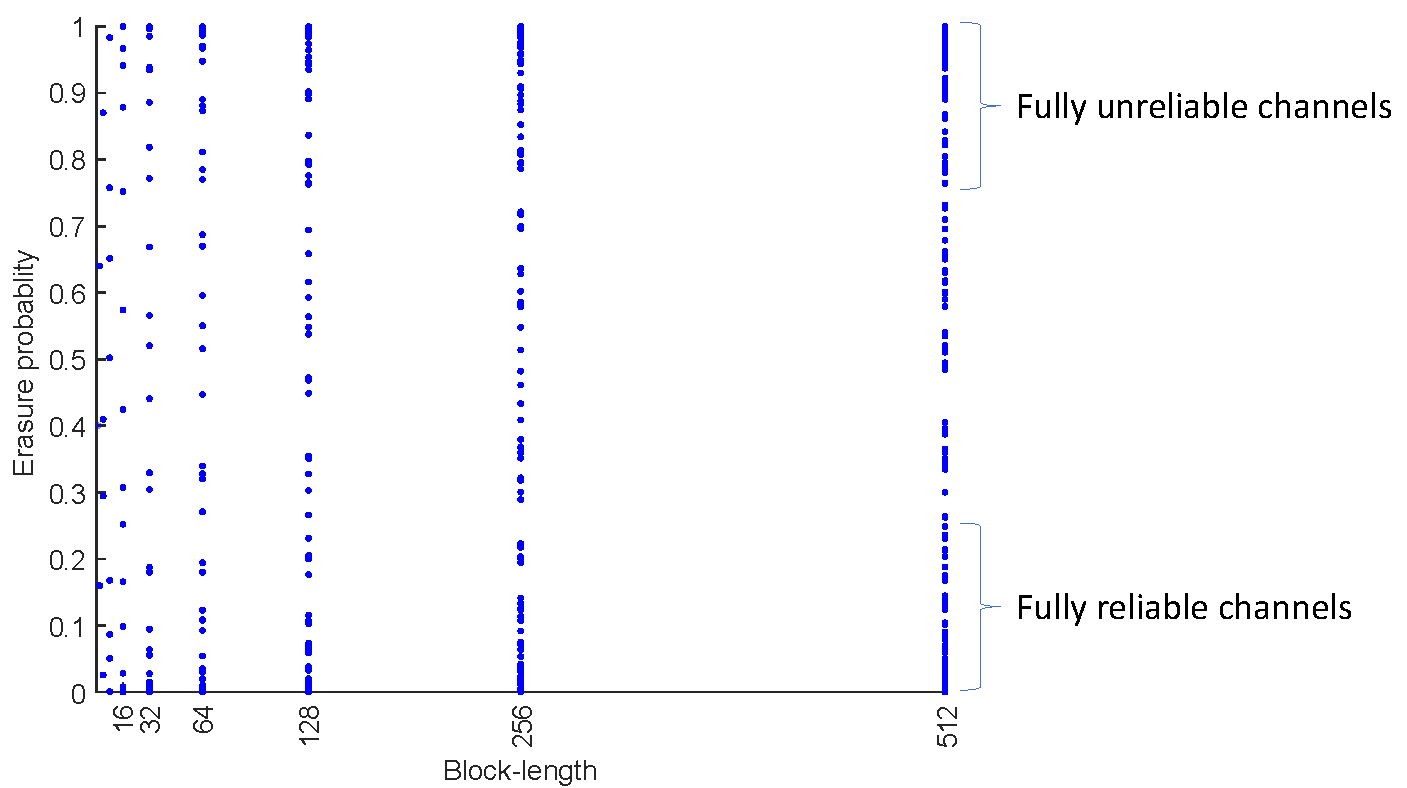
\includegraphics[width=1\textwidth]{./figures/channel_polarization_plot.pdf}
	\caption{Channel polarization example for binary erasure channel with $\epsilon = 0.4$}
	\label{fig:channelPolarizationPlot}
\end{figure}

Figure \ref{fig:channelPolarizationPlot} illustrates channel polarization for different block lengths for binary erasure channel with erasure probability $\epsilon = 0.4$. It can be seen that as block-length increases channels gets polarized to extremal channels (either completely reliable or unreliable).

\subsection{Encoding} \label{polarEncoding}
After polar code constructions, Out of $N$ bit positions information bits are placed in the most reliable bit indices position and non reliable bit positions are called frozen bits whose values are set to zero. This $N$-bit vector $U$ is multiplied with generator matrix obtained by the kronecker power of Arikan kernel matrix. Multiplying with generator matrix can also be represented as circuit form. Arikan kernel matrix can also be represented in circuit form as shown in figure \ref{fig:butterFlyCicuit} also called butter fly circuit.

\begin{figure}[h]
	\centering
	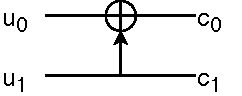
\includegraphics{./figures/ButterFlyCircuit.pdf}
	\caption{Butterfly circuit representing Arikan Kernel matrix}
	\label{fig:butterFlyCicuit}
\end{figure}

For $n = 3$ block length $N$ becomes 8 for such a case encoding circuit looks shown in  figure ~\ref{fig:encoderCircuit}, which is a repeated application of butter fly circuit. The read locations are the frozen bit indices which are set to zero, in remaining positions information bits are inserted. Output of the circuit is a code word which is transmitted over the channel. Lets consider an example with $N = 8$ and $K = 4$, rate of this code is $R = K/N = 1/2$. As given in the figure frozen bit indices are ${\{0,1,2,4\}}$ remaining indices contain information bits.  Let the information which needs to transmitted be \{1,1,0,0\}, then after placing information bits at reliable channel positions the vector $U$ becomes \{0,0,0,1,0,1,0,0\}. It is passed through the polar encoding circuit shown in Figure ~\ref{fig:encoderCircuit}. Result at the output of encoder is \{0,0,1,1,1,1,0,0\}. These encoded bits are then transmitted over the channel.

\begin{figure}[h]
	\centering
	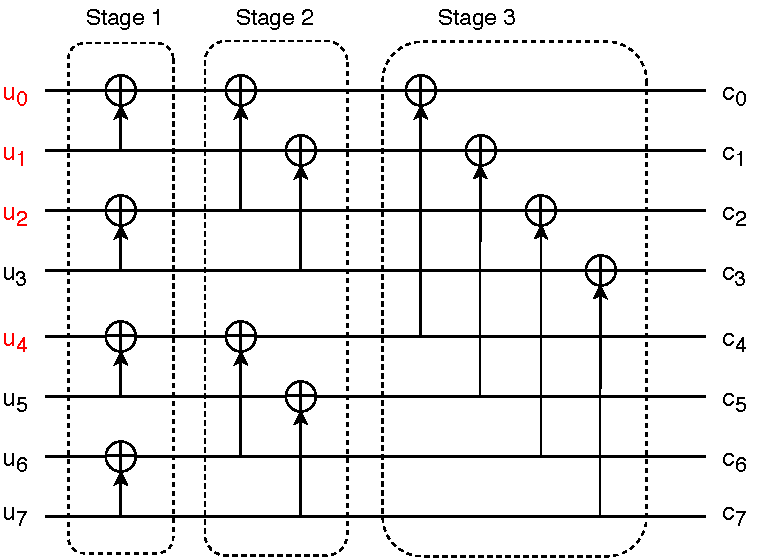
\includegraphics[width=0.8\textwidth]{./figures/EncodingCircuitStagesNew.pdf}
	\caption{Polar encoder in circuit form for $N = 8$}
	\label{fig:encoderCircuit}
\end{figure}

The encoding circuit is nothing but recursive application of the transformation represented by the butterfly circuit shown in the figure ~\ref{fig:butterFlyCicuit}. One butterfly unit can transform two uncorrelated bits $(a,b)$ into two correlated output bits $(a\oplus b,b)$ which is dominated by $k$ the Arikan Matrix. This corresponds to two channel polarization. In the above example reliability of the $u_{1}$ is increased compared to the $u_{0}$ channel. This operation recursively applied to the whole code word results in the circuit shown in the figure ~\ref{fig:encoderCircuit}. Code word splits into two parts in stage-3, which again splits into two parts in stage-2 and so on, until one reaches to single source bit $u_{i}$ in stage-1. So the process of polar encoding for $N = 8$ involves three stages of butterfly operations. Generally for a given code length $N=2^{n}$, the polar encoding consists of stages each with $N/2$ butterfly operations, which results in an encoding complexity of $O(N\log(N))$.


%\TODO{If you find any interesting, useful information for better understanding of the polar encoding, don't hesitate to include here.}

\subsection{Decoding}
As shown in section ~\ref{polarEncoding}, repetitive application of butterfly operation during encoding introduces correlation between the source bits. At the receiver, this is exploited to estimate the transmitted codeword. Utilizing the high correlation between the source bits forms the central idea behind the basic polar decoding algorithm called \emph{Successive Cancellation (SC)}. This method sequentially decodes each of the bits and takes previously estimated value to account for estimating the next bit. This sequential decoding exploits correlation between the source bits which as introduced during polar encoding process. Due to the sequential nature of SC decoding, the process has high. Improving the basic decoding algorithm has been the topic of researchers in academia and industry. These improvements are mainly directed towards two goals, first reducing decoding latency and second improving the error correction performance. Significant reduction in decoding latency is achieved by \cite{SSC} and \cite{fastSSC}. In these works, instead of decoding sequentially individual bit, special nodes are identified which can be decoded in parallel. Although polar codes are the first theoretically capacity achieving codes with explicit construction, their error correction performance at short block lengths is not comparable with that of LDPC or Turbo codes. This behavior can be better explained by the way decoding is performed. As presented earlier SC algorithm works by sequentially decoding individual bits and using information of previously decoded bits for estimating next bit. The issue with algorithm is if the previously decoded bit is wrong, then there is no way of correcting this bit.

To overcome this problem \cite{SCL} presents a improved version of the SC algorithm called Successive Cancellation List Decoding (SCL). The basic idea is instead of deciding a value of bit $u_{i}$ it takes both options, this results in two decoding paths for every bit, so to avoid exponential growth of complexity decoding candidates are restricted to $L$ the list size. At the end of decoding, most probable candidate is chosen from list. Performance of polar codes with SCL is still not as good as LDPC or Turbo codes at small and moderate block lengths. Polar code concatenated with CRC as outer code beats the LDPC codes of similar block length \cite{SCL}. SCL algorithm has a better error correction performance than SC, however it comes with a increased complexity and high decoding latency. Due to these reasons, in this work only fast-SSC algorithm is considered although its error correction performance is less than SCL.

\paragraph{\emph{A. Successive Cancellation Decoding (SC)}}  \label{SC}
The recursive SC decoder is basic algorithm presented in \cite{Arikan} for decoding polar codes.  SC decoder is inherently sequential, it estimates $\hat{u_{i}}$ of $u_{i}$ by using channel observation $y^{N}_{1}$ and all the previously decoded bits $\hat{u}_{1}^{i-1}$. If $u_{i}$ is frozen bit, the decoder assigns $\hat{u_{i}}$ to known value (mostly zero). If $u_{i}$ is an information bit, the decoder waits for all the previous bits to compute the decoding metric. It may be one of the three different type of metrics: \newline

$\bullet$ log-likelihood ratio (LLR) where


\begin{equation}
L_{N}^{(i)}(y_{1}^{N},\hat{u_{1}}^{i-1}) = \ln{\Bigg(\frac{W_{N}^{(i)}(y_{1}^{N},\hat{u_{1}}^{i-1}|u_{i} = 0)} {W_{N}^{(i)}(y_{1}^{N},\hat{u_{1}^{i-1}}|u_{i} = 1)}\Bigg)};
\end{equation}

$\bullet$ likelihood ratio (LR) where 

\begin{equation}
LR_{N}^{(i)}(y_{1}^{N},\hat{u_{1}}^{i-1}) = \Bigg(\frac{W_{N}^{(i)}(y_{1}^{N},\hat{u_{1}}^{i-1}|u_{i} = 0)} {W_{N}^{(i)}(y_{1}^{N},\hat{u_{1}^{i-1}}|u_{i} = 1)}\Bigg);
\end{equation}

$\bullet$ log-likelihood (LL) where 

\begin{equation}
LL(y_{1}^{N},\hat{u_{1}}^{i-1}) = \Big[ln\Big(W_{N}^{(i)}(y_{1}^{N},\hat{u_{1}}^{i-1}|u_{i} = 0)\Big), ln\Big(W_{N}^{(i)}(y_{1}^{N},\hat{u_{1}^{i-1}}|u_{i} = 1)\Big)\Big];
\end{equation}


Decoding metric computed from LLR's exhibit better numerical stability than those from LR's or LL's, so we have used the LLR's metric throughout this work. There are different ways to view and understand the operation of SC decoder. In this work decoding is viewed as message passing algorithm on an binary tree with $\log(N)$ levels. Decoding is performed by traversing a tree from root to leaf node. Process of decoding involves check node(CN), variable node (VN) operations and threshold detection at the leaf node. Decoder receives a LLR value for every bit which needs to be decoded (including both frozen and information bits), hence for a code with block length $N$, SC decoder receives $N$ LLR values. Decoding process estimates the bits $\hat{u}_{i} $  where $i = 0,1,2...,(N-1)$. The decoding tree for $N = 8$ looks as shown in the figure ~\ref{fig:decodingTree}.

\begin{figure}[h]
	\centering
	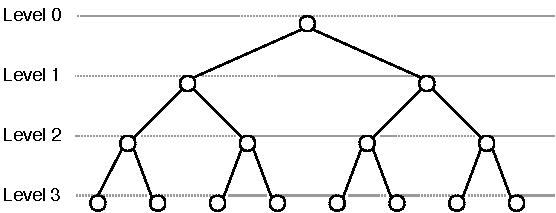
\includegraphics{./figures/decodingTree.pdf}
	\caption{Decoding tree}
	\label{fig:decodingTree}
\end{figure}

\begin{figure}[h]
	\centering
	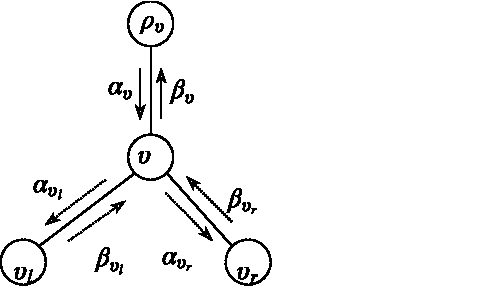
\includegraphics{./figures/messagePassingDiaS.pdf}
	\caption{Local Decoder}
	\label{fig:msgPassingDia}
\end{figure}

In a decoding  tree, the messages to left child node are computed with CN and to the right are with VN operation.  Figure ~\ref{fig:msgPassingDia} shows how the messages are exchanged in a local component decoder.

The CN and VN operations in LLR domain are given by following equations:

$\bullet$ Check Node (CN) operation

\begin{equation} \label{cnop}
	\alpha_{v_{l}}[i] = \alpha_{v}[i] + \alpha_{v}[i + N_{v}/2]
\end{equation}

$\bullet$ Variable Node (VN) operation

\begin{equation} \label{vnop}
\alpha_{v_{r}}[i] = \alpha_{v}[i + N_{v}/2] + (1 - 2\beta_{v_{l}}[i]) * \alpha_{v}[i]
\end{equation}

After decoding is done at both right and left child nodes the bits are combined at common parent node. the bit combining operation is given by the following equation.

\begin{equation*} \label{bitCombination}
\beta_{v}[i] = \begin{cases}
				\beta_{v_{l}}[i] \oplus \beta_{v_{r}}[i] & \text{if }i < N_{v}/2 \\
				\beta_{v_{r}}[i]
				\end{cases}
\end{equation*}

In the figure ~\ref{fig:msgPassingDia} and in equations ~\ref{cnop}, ~\ref{vnop}  $\alpha_{v}$, $\beta_{v}$ represent intermediate LLR values and estimated bits at the local decoder respectively.

Figure \ref{fig:scDecodingEg} gives an example of SC decoding for block-length $N=8$ and number of information bits $K=4$. In the figure decoded bits and intermediate $\beta_{v}$ are represented by black font color and computed intermediate $\alpha_{v}$ are indicated by green. Frozen pattern is provided below the leaf nodes. Frozen pattern indicates position of information and frozen bits. One in frozen pattern indicates frozen bit, zero indicates information bit.

\begin{figure}[h]
	\centering
	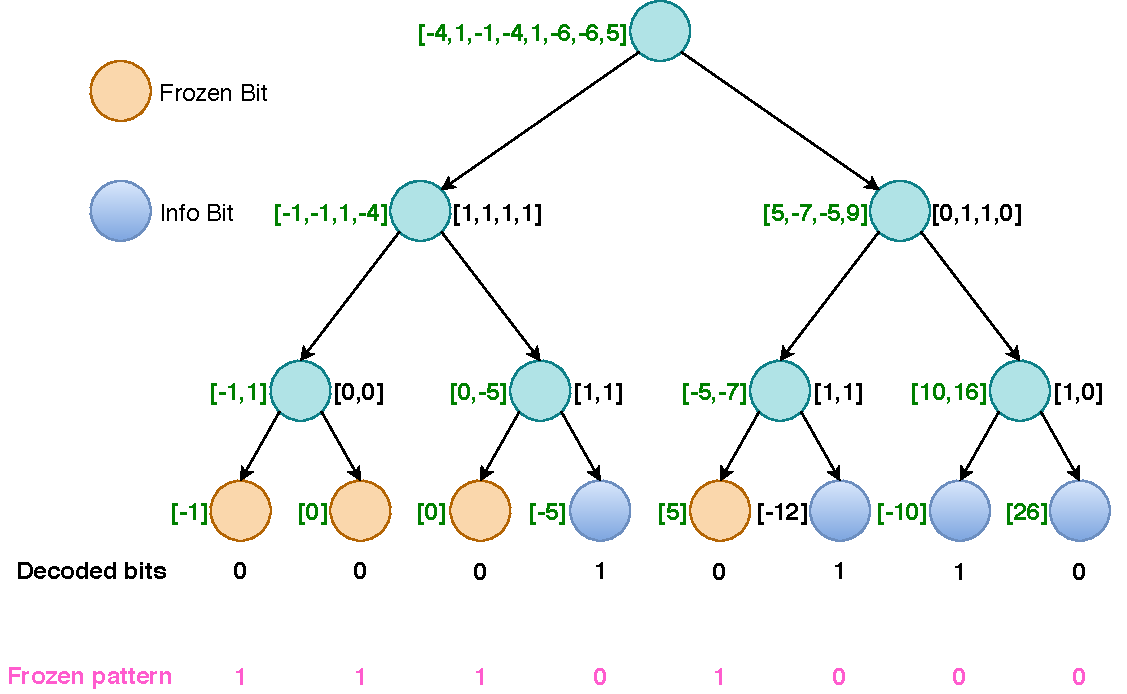
\includegraphics[width=0.9\textwidth]{./figures/SCDecodingExample.pdf}
	\caption{SC decoding example}
	\label{fig:scDecodingEg}
\end{figure}

%\TODO{provide an example of decoding with real LLR values for $N = 8$}

\paragraph{\emph{B. Improved Successive Cancellation Decoding (fast-SSC)}\newline}  \label{fastSSC} 
In basic SC algorithm, decoding is performed sequentially, previously decoded values are used for decoding the present bit. Due to sequential nature of the decoder, decoding latency is high.\cite{SSC} and \cite{fastSSC} try to identify special kind of nodes in a decoder tree which can be immediately decoded without traversing till the end of the tree. \cite{SSC} tries to identify node with all information bits or all frozen bits. These nodes are called rate-one($R1$) and rate-zero ($R0$) nodes respectively. The $R1$ node can be decoded by taking hard decision and polar transform, since there is no extra information which can be gained from traversing the tree. Decoding of $R0$ node is not necessary since none of them are information bits, so all the bits are set known value which is known at transmitter and receiver which are mostly set to zero. \par Authors in \cite{fastSSC} extend the idea presented in \cite{SSC} by identifying two more kind of special nodes which can be decoded without traversing the tree single parity check ($SPC$) and repetition ($REP$) nodes. Both in \cite{SSC} and \cite{fastSSC} node type is identified based on the frozen pattern at the component decoder. For $SPC$ node, only one frozen bit is present at left most position. For $REP$ node, frozen pattern contains one information bit at right most position, remaining are frozen bits.

One such example, when frozen indices for $N = 8$ are $\{0,1,3,4\}$. The full decoding tree of Figure ~\ref{fig:decodingTree} gets reduced to a tree with fewer nodes as shown in Figure ~\ref{fig:decodingTreePruned}. We can easily see that, in the original decoder tree number of nodes were $15$, in the pruned tree nodes are reduced to 7, which results in a significant reduction in number of computations and decoding latency.

\begin{figure}[h]
%	\centering
	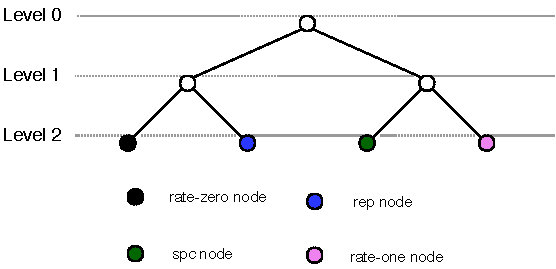
\includegraphics{./figures/decodingTreePruned.pdf}
	\caption{Pruned Decoder Tree}
	\label{fig:decodingTreePruned}
\end{figure}


%\paragraph{\emph{C. List Decoding of Polar Codes (SCL)}\newline}  \label{SCL}


%Here I need to explain the typical features which are important for understanding the latency contributors and how they can be resolved
\section{Processor architecture background}
To better understand the bottlenecks and optimizations performed in software implementation of 5G FEC chain, it is necessary to understand the fundamentals of processor architecture. This section gives necessary background about cache memory systems, instruction pipelining, branch predictors, Vector processing units and recursive function calling mechanism.

\subsection{Cache memory} \label{cacheSection}
In the modern processors, fast memory called cache is used to reduce the average access time of main memory also called RAM (Random Access Memory). Cache minimizes the number of accesses to RAM by storing frequently accessed location's data in it, hence avoiding huge penalty of reading data frequently from RAM which operates at a much lower frequency than the CPU. When memory location is accessed for the first time it is copied from RAM to cache, future accesses to same location is done via cache. These fast memory is placed between RAM and processor. In modern processors instead of single cache, multi-level caches are present. The main idea behind having multi-level caches is that if the data is not found in first level then second level is checked if not then third level until the last level, still if the data is not found then RAM is accessed. This model significantly reduces the probability of accessing the RAM compared to having a single level cache. Complete memory hierarchy of the modern processors is shown in the figure  ~\ref{fig:memoryHierarchy} \cite{CMP}.

\begin{figure}[h]
	\centering
	
\includegraphics[width=0.7\textwidth]{./figures/memoryHierarchy.pdf}
	\caption{Memory Hierarchy}
	\label{fig:memoryHierarchy}
\end{figure}

Above figure shows processor architecture with three level caches namely L1, L2 and L3. In the order of increasing access latency, reducing cost and increasing size. L1 cache is fastest, costliest and smallest among all caches. Data is mapped to either memory or registers. If the available registers are not enough in such a case data is stored in memory. If the data is not found in all cache levels then it results in cache miss which causes processor instruction execution to stop until data is fetched from RAM. Whenever the memory location is accessed for the first time it always results in cache miss. Present data modern processors provide special instructions to avoid these compulsory cache misses, these are called cache prefetch instructions which allow programmer to fetch data from cache before it is accessed, hence hiding the memory access latency. Some other software techniques to reduce cache misses are reusing the allocated memory as much as possible and bit packing/unpacking to reduce the required memory. In this work, all the above mentioned techniques namely using prefetch instructions ($\mathtt{PREFETCH}$) provided by AMD EPYC processor, reusing the allocated memory and bit packing/unpacking are used reduce the memory access latency.

\subsection{Instruction pipelining and branch predictors}
Traditionally processors were designed to follow the steps fetch, decode, execute, memory finally write-back and then fetch the next instruction. Although these steps are sufficient to solve any problem in hand, it is very inefficient in terms of hardware utilization. When instruction is getting fetched, remaining modules are idle, if instruction is in decode phase remaining modules are idle similarly other phases. To overcome under utilization of hardware resources modern processors implement instruction pipelining concept, where if the current instruction is in decoding phase the next instruction will be concurrently fetched by the fetch module. Pipelining mechanism increases the instruction throughput by significantly reducing CPI (Cycles per Instruction). Example of sequential and pipelined execution is shown in figure \ref{fig:pipeline} \cite{SoCT}.

\begin{figure}[h]
	\centering
	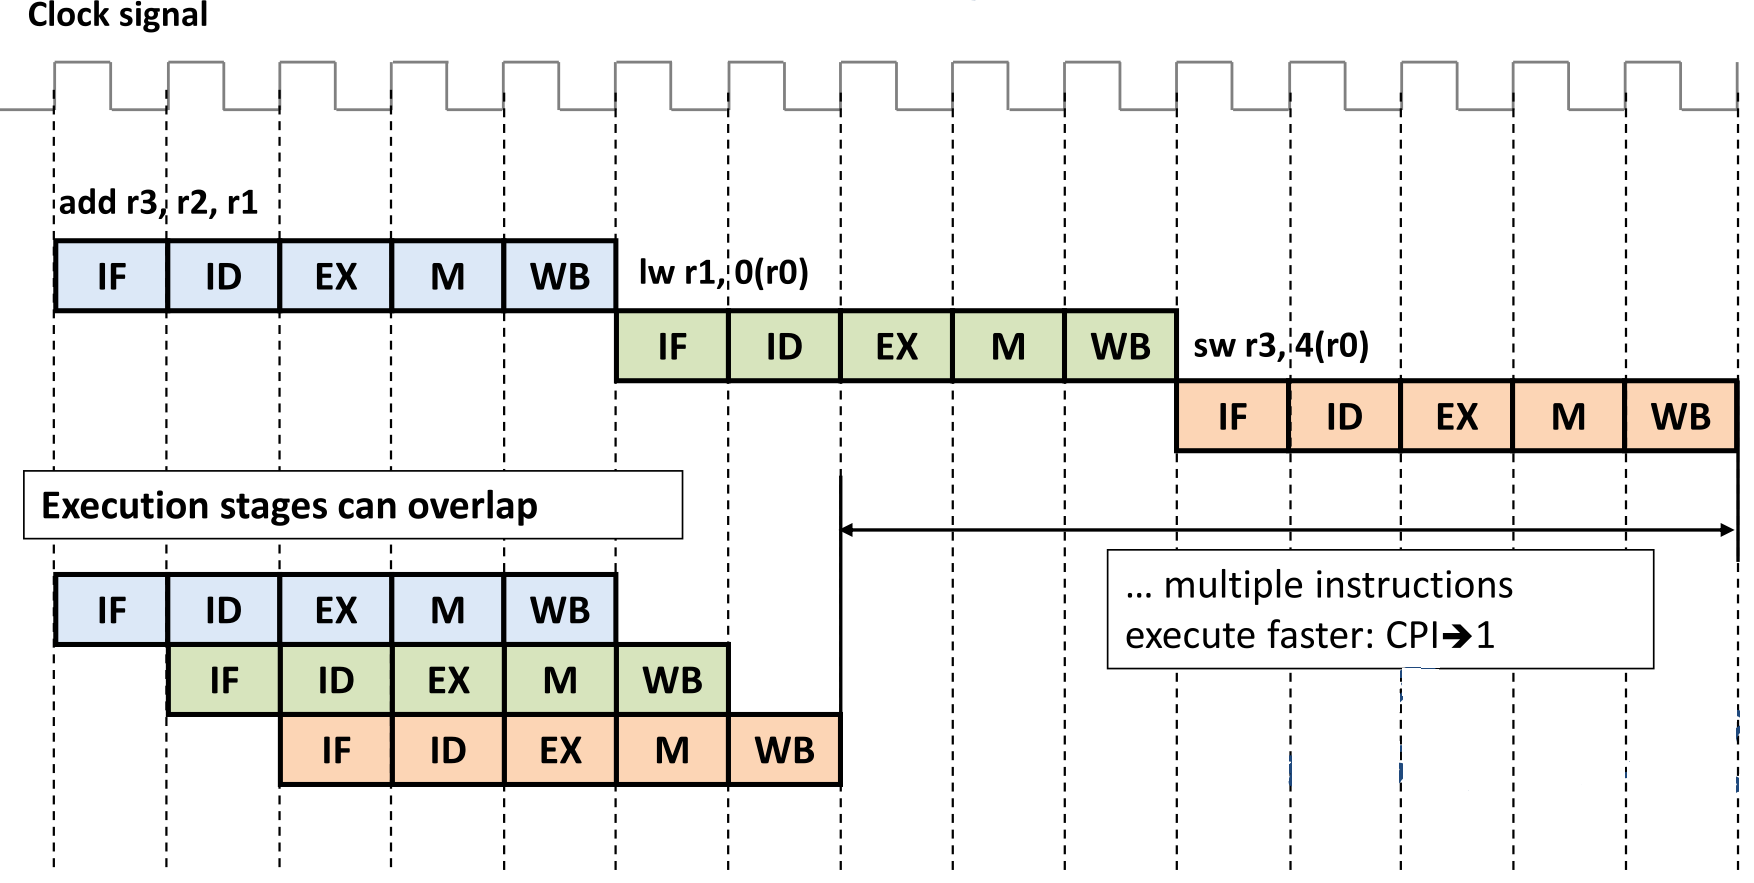
\includegraphics[width=0.9\textwidth]{./figures/pipeline_seq2_edited.pdf}
	\caption{Instruction pipelining}
	\label{fig:pipeline}
\end{figure}

Example shown in figure \ref{fig:pipeline} assumes only five phases of instruction execution. Modern processors divide instructions execution to nineteen plus phases, which allows running processor at much higher frequency due to reduced critical path delay. Maximum advantage of pipelining can only be exploited when there are no pipeline stalling or flushing which happen when there is a data dependency, cache misses or branch instructions. Major contributors to pipeline stalling are cache misses and branch instructions. As explained in \ref{cacheSection} can be reduced by using combination of different optimization techniques. Next culprit is branch instructions, whether to branch or not is decided only the at execution stage. By the time branching is decided, many of the future instructions are already fetched, if the decision is to jump then all the prefetched instructions must be flushed which introduces stall in the pipeline. To overcome this issue branch predictors are designed to pro-actively fetch instructions from correct address, hence avoiding flushing of pipeline. Branch predictors function by storing the previous decisions on the branching whether it was taken or not, hence requires correct previous state to pro actively fetch future instructions. This method reduces the pipeline caused due to looping type of code, by reducing pipeline flushes. For the scenarios where there are no looping instruction just if or if-else constructs branch predictors fail to correctly fetch the future instructions. These kind of scenarios can be minimized by avoiding branch instructions wherever possible and by providing hints to compiler built-in macros to reduce the branching by better placement of assembly instructions (kind of instruction scheduling). One such macro is 
\begin{minted}{c++}
	long __builtin_expect(long EXP, long C); 
\end{minted}
which tells compiler to place more frequently executing part of the code just after branch instruction to minimize pipeline flushing. Code snippet \ref{code:likelyHint} shows the typical usage.

\begin{code}
	\captionof{listing}{Branching hints to compiler}
	\label{code:likelyHint}
\begin{minted}{c++}
#define likely(expr) __builtin_expect(!!(expr), 1)
if (likely(a > 1)) {
	//Frequently executing part, most of the cases a is greater than 1
	...
} else {
	//Rarely executing part, rarely a is less than 1
	...
}
\end{minted}
\end{code}

Another feature provided by modern processors is conditional move instruction ($\mathtt{CMOV}$). Compiler intelligently maps if statements to conditional move instructions. $\mathtt{CMOV}$ copies a particular value to register or memory based on the flags set. It is not vulnerable to branch-prediction failure since no branch instructions gets generated, hence avoiding pipeline flushing. Following listing in \ref{code:NaiveCMOVEg} and \ref{code:CMOVEEg} illustrates the feature.

\begin{code}
	\captionof{listing}{Naive method}
	\label{code:NaiveCMOVEg}
\begin{minted}{c++}
uint32_t bitMask = 0;
if(CRCLENGTH == 6) //If Crc6 needs be calculated, then change the mask.
  bitMask = 0x3F;
else
  bitMask = 0x7FF;
\end{minted}
\end{code}

\begin{code}
	\captionof{listing}{With $\mathtt{CMOV}$}
	\label{code:CMOVEEg}
\begin{minted}{c++}
uint32_t bitMask = 0x7FF; //Initializing with CRC11 mask.
if(CRCLENGTH == 6) //If Crc6 needs be calculated, then change the mask.
  bitMask = 0x3F;
\end{minted}
\end{code}

Both code achieve same results, however \ref{code:NaiveCMOVEg} pipeline flush will happen due to branch-misprediction, for \ref{code:CMOVEEg} compiler identifies conditional move construct and generates $\mathtt{CMOV}$ potentially avoiding pipeline flush. Optimizations such as minimizing branches, using built-in macros and using constructs which help compiler to identify pattern are utilized in this work.

\subsection{Vector processing units}
Vector processing units are special kind of multiple computational elements that perform same operation on multiple data points simultaneously. Machines with vector processing units exploits data level parallelism but not concurrency. Same instruction operates on multiple data points in other words there are simultaneous computations but there is a single process. These special kind of instructions are also called SIMD (Single Instruction Multiple Data) in Flynn's taxonomy of parallel computers. These instructions are particularly useful when same operation needs to applied set of data, for example scaling a vector by constant. SIMD units can be thought of same processing unit replicated multiple times which are operated by a single instruction. Figure \ref{fig:simdUnits} from wikipedia \cite{SIMDWiki} illustrates the concept of SIMD and how single instruction pool operates on multiple data points.

\begin{figure}[h]
	\centering
	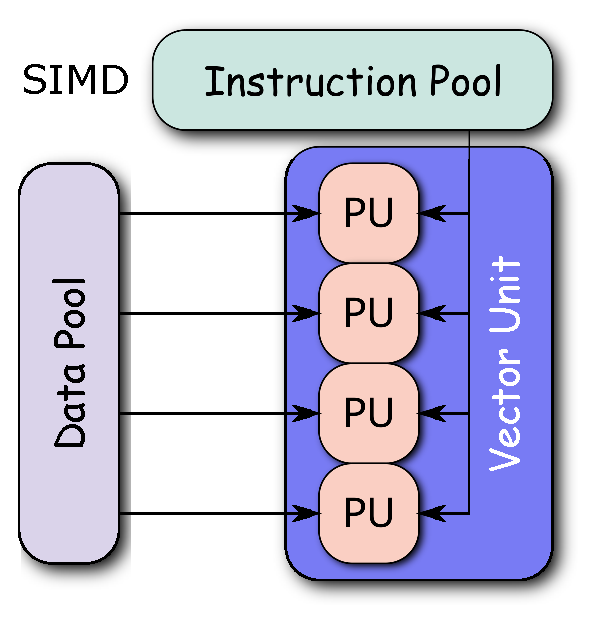
\includegraphics[width=0.5\textwidth]{./figures/SIMD2.eps}
	\caption{Vector processing units}
	\label{fig:simdUnits}
\end{figure}

Modern x86 processors from AMD and Intel provide different SIMD extensions named SSE (Streaming SIMD Extensions), AVX (Advanced Vector Extensions) with register size of 128-bits, AVX2(Advanced Vector Extensions 2) with register size 256-bits and the latest AVX-512 with register size 512-bits. In this work AMD EPYC processor used which provides SSE, AVX and AVX2 instructions, implementation is carried out using the features available in these extensions.

\subsection{Recursive function calling mechanism}
Most of the encoder and decoder implementations are implemented through recursion. Recursive function is a method which calls itself. It is a powerful tool in computer science which can be used for solving many interesting problems. However when it comes to performance, recursive problem solving falls behind algorithms which use looping to solve the same problem. Mainly due to the fact that every time a recursive function is called new stack frame is allocated, local data is pushed to call stack and execution must branch to the beginning of function. Branching and pushing data to call stack are expensive operations. In case of polar codes both encoding and decoding are implemented as recursive functions. To reduce the latency of FEC chain encoding/decoding implementations are unrolled to avoid recursions. For encoder, unrolling is carried out by manually implementing multiple inline functions. In decoder implementation unrolling is carried out by using C++ template concept. Although unrolling increases code size, for the application in hand latency is of at most importance than code size. Unrolling of the encoder and decoder implementations significantly improved the latency of FEC chain. % Background about polar codes and their usage in 5G.
        \chapter{Encoding FEC Chain} \label{chap:encoder}

% In this document explain all the things which I have done until the midterm presentation.
% All the details, Optimization techniques I have employed.
% Following text might be useful for writing the text.
% Also my midterm presentations/office presentations will be really useful for writing this part.  
% Reference paper for explaining the different components of the this FEC chain "Design of Polar codes for 5G NR radio"

%Work I have done Until now.
%
%%****************Optimizations to the original implementations until now.
%%****************Generic optimizations
%- Using optimization primitives such as likely and unlikely.
%- Aligning memory to 32 bytes so copying of data can be vectorized.
%- Polar transform optimization	
%- Replace binary additions with xor. instead of addition and then modulus two.
%- division and multiplications by left and right shift operations.
%- Avoided copy operations in polarTransform operations.
%****************Optimization in getting reliability indices.
%- Avoided remove and erase operations which have huge overhead. Wrote a efficient mechanism(reduced the latency by 176 us).
%- Instead removing and erasing I mark the element as removed.
%- Since the reliability indexes won't change. I built a look up table in place of searching all (1024)indices reduced the latency by 40us
%- Avoided copying operations of interleaved indexes.
%- Unrolled the loop to reduce the jumps.
%****************Rate matching optimizations.
%- optimization in subblock interleaving, Rewrote the logic to avoid E number of division and modulus operations.
%- Unrolled the for loops in subblock inteleaving method.
%- Implemented optimal version of bit selection, Avoided E number of modulus operations which are very costly.
%- Again optimization primitives for helping the branch predictor.
%
%
%Fast version of Encoding API's.
%In the original implementation of the polar encoding each of the bit is treated as 32 bit integer. This is highly inefficient
%when the goal is to process multiple bits at time. With each bit considered as 32 bit integer SIMD instructions won't provide
%any performance improvement. Reason is SIMD instruction can process multiple bits at time. avx2 instructions 256bits at a time.
%if we have 32 bits to represent a single bit. we can process only 8 bits at time. Which doesn't significantly improve the
%performance. To avoid this disadvantage and make use of SIMD capability. each 64 bit integer is considered as 64 bits of data.
%so one avx2 instruction can process 256 data bits in a single instruction.
%- Built a look up table to avoid last eight stages of polar encoding instead of traversing till end of tree.
%- Implemented SIMD instruction based encoding. Encoding happens within 0.6 us for N = 512.
%- Implemented optimal version of CRC calculation which can calculate CRC for PDCCH chain within 0.8 us. Original implementation was taking 7 us.
%- Implemented a bit interleaver which can deal with this format of data.

In this section, complete polar encoding FEC chain used in 5G is explained. Methods used for code profiling and latency measurement are presented. After figuring out the latency contributors code optimization/algorithm optimizations employed during the FEC chain development are presented and then presents how SIMD feature of the modern processors is exploited to obtain the low latency for PBCH and PDCCH FEC chains and frozen set selection algorithm improvement with the aid of look up table, finally presents the encoding process as traversal of a binary tree and how the encoding latency can be improved by pruning the tree hence avoiding the tree traversal instead using a lookup table to obtain the encoded result.

In 5G framework, Polar codes are used in downlink to encode downlink control information (DCI) over physical downlink control channel (PDCCH) and for payload in physical broadcast channel (PBCH). In uplink, to encode uplink control information (UCI) over the physical uplink control channel (PUCCH) and the physical uplink shared channel (PUSCH). In this work, notations introduced in 3GPP technical specification\cite{3gpp.38.212} are used.

The figure ~\ref{fig:5g_fec_chain} represents the complete polar FEC chain for PBCH and PDCCH in downlink. Let's look at each of the components briefly to understand the FEC chain. In general $A$ bits have to be transmitted over a code of length $E$ code bits. $L$ CRC bits are added to the information bits, resulting in  $K = (A + L)$ bits. These $K$ bits are passed through an interleaver. Interleaved bits are concatenated with a parity bits and assigned to information set to obtain a vector $\boldsymbol{u}$. Encoding is done with a mother code with parameters $(N,K)$, with $N = 2^{n}$. Encoding is performed $\boldsymbol{d = uG_{N}}$ the generator matrix $\boldsymbol{G_{N} = G^{\otimes n}}$ obtained by $n^{th}$ kronecker product of Arikan matrix. Encoded codeword $\boldsymbol{d}$ passed through a subblock interleaver which divides the codeword in to blocks of 32 bits and performs interleaving between them according to 32 integers (interleaving pattern is nothing but a bit reversal of bit position) shown in figure. \TODO{add picture of bit reversal operation}. After subblock interleaving is completed rate matching is carried out. To map $N$ to $E$ bits. Rate matching can repetition, puncturing or shortening. This decision is taken based on the value of $E$, $N$ and $K$. Finally to improve the error correction performance channel interleaving is done. This section of the report presents  implementation details of each of these operations in an algorithmic level with small code snippets whenever necessary. Analyzes latency introduced by different sections of FEC chain and also presents the algorithmic and platform specific optimizations.

\begin{figure}[h]
	\centering
	\includegraphics[width=0.7\textwidth]{./figures/5GFECChain.pdf}
	\caption{Polar Encoding FEC chain for PDCCH/PBCH}
	\label{fig:5g_fec_chain}
\end{figure}

\section{Data packing and Unpacking Operations} \label{dataPackUnpack}
Typically in software implementations, for clarity and ease implementation each bit of information is represented with 32-bit or 64-bit integers. Due to the presence of only one bit of information in each integer if want to encode/decode 1024 bits, then 1024 integers are involved in encoding/decoding process. However this isn't the case in hardware implementations since each bit can be processes in Harware Description languages (HDL). Representing each one bit of information using 32/64-bit integer has following disadvantages. 

\begin{description}[font=$\bullet$~\normalfont]
	\item Increased memory footprint: If one decides to represent each bit using 64-bit integer for 1024 bits of information 64*1024 bits memory needs to allocated which equivalent to 8 kilobytes. Allocating and initializing this memory can introduce significant latency.
	\item Results in more cache misses: If more memory is allocated then more data needs to accessed from DRAM which can result in significant number of cache misses.
	\item Serializes encoding/decoding: General purpose processor's have a data path width of 64-bit. If each bit is represented using 64-bit integer we are not using capability of processing 64 bits simultaneously instead each bit is processed sequentially. This can make encoding/decoding sequential although processor is capable of processing multiple bits in parallel.
\end{description}

To avoid these disadvantages and to enable data parallelism, this implementation of encoder tries to pack the multiple information bits to one integer. Although packing information bits to single integer has advantages, for some operations such as bit wise interleaving accessing each bit efficiently is very important. To exploit the advantages of bit packing as well as the advantages of each bit as integer, it is necessary to convert between the two. This is where the power of SIMD instructions in modern processors come to rescue. These processors come with special hardware instructions which help to efficiently pack and unpack data. Information bits are used in packed format when data parallelism needs to exploited and in unpacked format when certain operations require bits to accessed individually. These pack/unpack instructions are very efficient with low latency.

Some examples of these instructions are:
\begin{lstlisting}
	int _mm_movemask_pi8(__m64 a);
	int _mm_movemask_epi8(__m128i a);
	__m256i _mm256_unpackhi_epi8(__m256i a, __m256i b);
	/** many more **/
\end{lstlisting}

\TODO{May be give examples code snippet which packs and unpacks bits in an efficient manner.}

\TODO{cite to agner fog optimization manuals. \cite{AgnerFog}}

\section{CRC calculation}
%Explain why CRC attachment is considered in whole FEC chain, how it is useful for decoding polar codes. Explain algorithmic complexity of CRC calculation, How much time it was taking, How the optimization is carried out to reduce the CRC calculation time.
As shown in the figure \ref{fig:5g_fec_chain} L-bit CRC is calculated for $A$ information bits and attached as part of message. Number of CRC bits (L) varies for different physical channels. In downlink, for payload of PBCH/PDCCH 24-bit CRC is used. Uplink Control Information (UCI) uses 6-bit or 11-bit CRC based on the value of $A$. For $12 \leq A \leq 19$ and $A \geq 20$ 6-bit CRC and 11-bit CRC are used respectively. Polynomials use for different CRC values is shown below \cite{3gpp.38.212}.

\begin{equation} \label{crc_polynomial6}
g_{6}(x) = x^{6} + x^{4} + 1
\end{equation}
\begin{equation} \label{crc_polynomial11}
g_{11}(x) = x^{11} + x^{10} + x^{9} + x^{5} + 1
\end{equation}
\begin{equation} \label{crc_polynomial24}
g_{24}(x) = x^{24} + x^{23} + x^{21} + x^{20} + x^{17} + x^{13} + x^{12} + x^{8} + x^{4} + x^{2} + x + 1
\end{equation}

Information bits concatenated with CRC increases the error correction performance of polar codes significantly. CRC is be used for selecting the correct code word out of potential candidates when employing a list-decoding algorithm. With CRC aided decoding, polar codes performance is very close maximum likelihood decoding. To reduce the latency of encoding FEC chain CRC needs to calculated very efficiently. One of the naive implementation of CRC calculation is, by using shift register method, which calculates CRC sequentially for one bit at a time as given in \cite{naiveCRCCalculation}. As explained in the section \ref{dataPackUnpack}, it is very inefficient to process bits sequentially. Instead one can calculate the CRC blockwise with the help of lookup table. In otherwords, divide the data into blocks of $B$-bits, read the corresponding CRC value from lookup table and combine individual CRC's of blocks in an predefined way to create a CRC for complete data. Algorithm in \cite{Sarwate:1988:CCR:63030.63037} is adopted to calculate CRC24 using lookup table based approach. Data bits are divided into blocks of 8-bits and packed into 8 bit integers. CRC value corresponding to 8-bit integer is read from lookup table and combined with CRC of subsequent 8-bit integer, this process continues until CRC of data bits is completed. If the number of data bits are not multiple of 8 then zero's are appended at MSB position.  Table \ref{tab:crcLatencyTable} presents the latency values of naive and optimized  CRC calculation methods for payload of 41-bits on AMD EPYC processor running at 1.6 GHz with Turbo disabled. There is significant improvement in the optimized method compared to naive implementation.

\begin{table}[h!]
	\begin{center}
		\caption{CRC24 calculation latency comparison}
		\label{tab:crcLatencyTable}
		\begin{tabular}{c|c|c} % <-- Alignments: 1st column left, 2nd middle and 3rd right, with vertical lines in between
			\textbf{ } & Naive & Optimized \\
			\hline
			Latency ($\mu$s) & $7.7$ & $0.016$\\
		\end{tabular}
	\end{center}
\end{table}

\section{Input Bit Interleaver}
\TODO{Any optimization carried out in here, need to be explained clearly, Why this input bit interleaver is necessary. How much time this function takes.}

\section{Polar code construction}
The next step in the polar FEC chain in 5G is polar code construction. This step determines the error correction performance. Polar code construction is the process of identifying information and frozen bit position, i.e K out of N positions. There are many methods in the literature to construct polar codes. The inventor of polar code Arikan \cite{Arikan} proposed using Bhattacharyya parameter as reliability metric for Binary Erasure Channels (BEC) then deriving reliability values using Monte Carlo simulation. For other channels, Mori and Tanaka \cite{MoriTanakaDE} use more accurate density evolution (DE) methods but suffers huge complexity. Tal and vardy proposed Gaussian Approximation (GA) to reduce the complexity of DE with approximations. Still the GA method has high computational complexity which scales linearly with code block-length, and therefore unacceptable for varying SNR, block-length and code rate. In use cases such as 5G, where channel is continuously varying. it is not feasible to construct polar codes on the fly due to the complexity and stringent latency requirements of encoder and decoder. Polar code construction in 5G takes a suboptimal approach, instead of constructing polar codes for every different SNR, block-length and code rate, construction is carried out in such a way that code performs sufficiently good over large range of SNR, block-length and code rate. 5G polar code construction method is a contribution from Huawei which uses a $\beta$-expansion method with universal partial order (UPO) property of channel reliability as presented in \cite{betaExpansion}.

5G standard has adopted five different block-lengths polar codes. Block-length sizes $\mathcal{B}$ is given by $\mathcal{B} = \{32,64,128,256,512,1024\}$.
For each of the block lengths reliability indices values are specified in \cite{3gpp.38.212}. Polar code construction is straight forward when rate matching output $E$ greater than or equal to block length $N$, In such a case code construction involves selection of $K$ most reliable indices for information bits remaining positions are frozen. When rate matching output size $E$ is smaller than block-length $N$ reliability indices selection

\subsubsection*{5G polar code construction example for $N = 32, K = 16$ and $E = N$} \label{E_greaterThan_N}
Let's take an example with $N = 32$ channel reliability values are extracted from the reliability table provided in \cite{3gpp.38.212} and are given by

\begin{eqnarray*}
Q_{0}^{31} = \{ 0, 1, 2, 6, 3, 7, 9, 16,4, 8, 11, 17, 13, 19, 20, 26, 5, 10, 12, 18, 14, 21, 24, 27, 15, 23, 22, 28,\\
25, 29, 30, 31 \}
\end{eqnarray*}

The bit positions in reliability array $Q_{0}^{31}$ are ordered in increasing order of their reliability. For encoding with parameters $N = 32$ and $K = 16$, K most reliable indices in the array i.e last 16 indices are used as information bit positions 

\begin{eqnarray*}
	Q_{\textit{I}}^{\textit{K}} =  \{5, 10, 12, 18, 14, 21, 24, 27, 15, 23, 22, 28,25, 29, 30, 31 \}
\end{eqnarray*} 

There can be three cases with rate matching, $E > N$, $E == N$ and $E < N$ each of the cases requires different rate matching scheme, repetition, no rate matching and puncturing or shortening respectively. For the first case, due to no puncturing or shortening reliability values of bit channels are not affected after rate matching. Simplest case in polar code construction is when $E \geq N$. In this scenario no puncturing or shortening required.  In 5G FEC chain, it is not uncommon to have scenarios with rate matching output $E$ is less than block-length $N$. In such scenarios some bits need to discarded in rate matching stage through puncturing or shortening. Empirically its been observed for polar codes that at low rates puncturing works better and shortening for high rates \cite{lowcomplexityPuncShorteng}. When encoded bits are discarded in the rate matching stage reliability of bit channels get affected, identification reliable bits by taking effect of rate matching procedure makes polar code construction complex in terms of time. Functional implementation of reliability indices selection algorithm provided in \cite{3gpp.38.212} is carried out in C++ as given  ~\ref{algo:polarCodeConstuctionAlgo}. Upon code profiling of encoder FEC chain implementation, it was found that polar code selection algorithm is the most time consuming part among all the FEC chain stages. \newline

Following algorithm gives provides a simplified picture of function implementation to select information bit indices by taking the effect of rate matching. 
Notations used in the algorithm are same as the ones specified in 5G standard \cite{3gpp.38.212}.

$J(n)$ : Subblock interleaver pattern for a particular block-length $N$. \newline
$E$    : Rate matcher output size. \newline
$N$	   : Mother code block length. \newline
$K$	   : Number of information bits.\newline
$Q_{\textit{0}}^{\textit{N-1}}$ : Reliability indices array for block-length $N$ in ascending order of reliability. \newline
$\overline{Q}_{\textit{F}}^{\textit{N}}$ : Information bit positions. \newline


\IncMargin{1.5em}
\begin{algorithm}[H]
	\KwData{$Q_{\textit{0}}^{\textit{N-1}}$,$N$, $K$, $E$ and $J(n)$}
	\KwResult{$\overline{Q}_{\textit{I}}^{\textit{K}}$}
	$\overline{Q}_{\textit{F}}^{\textit{N}} = \emptyset$ \;
	\If {$\big(E < N\big)$} {
		\If {$\big((K*16) \leq (E*7)\big)$} {   %-------------------------------------------------> Puncturing
			$J_{sorted}(n) = sort(\{J(0),J(1),J(2)....J(N-E)\})$\;  \label{line:subblockRef1}
			\If {$\big(E \ge (0.75*N)\big)$} {
				$size = \ceil*{\big[(3*N*2 - E*4)/8\big]}$\;
				$\overline{Q}_{F}^{N} = J_{sorted}(n) \cup \{0,1,2, ... ,size-1\}$ \label{line:subblockRef2}
			} \Else {
				$size = \ceil*{\big[(9*N*4 - E*16)/64\big]}$\;
				$\overline{Q}_{F}^{N} = J_{sorted}(n) \cup \{0,1,2, ... ,size-1\}$ \label{line:subblockRef3}
			}	
		} \Else {							    %-------------------------------------------------> Shortening
			$\overline{Q}_{F}^{N} = \{J_{sorted}(E), J_{sorted}(E + 1), ... J_{sorted}(N-1)\}$ \label{line:subblockRef4}
		}
	}
	$frozenSize = \big|\overline{Q}_{F}^{N}\big|$ \;
	$infoSize = N - frozenSize$ \;
	$Q_{\textit{I}}^{\textit{N}} = Q_{\textit{0}}^{\textit{N-1}}$ \;
	
	\For{$i=0$ to $frozenSize$} {
		$iterator = remove(Q_{\textit{I}}^{\textit{N}},\overline{Q}_{F,i})$ \;
		$erase(Q_{\textit{I}}^{\textit{N}},iterator)$ \;
	}
	$startIdxInfo = N - K - n_{PC}$ \;
	$\overline{Q}_{\textit{I}}^{\textit{K}} = \{Q_{\textit{I,startIdxInfo}},Q_{\textit{I,startIdxInfo + 1}},...,Q_{\textit{I,END}}\}$
	\caption{Polar code construction}
	\label{algo:polarCodeConstuctionAlgo}
\end{algorithm}
\DecMargin{1.5em}

Above algorithm shows how the information bit indices are selected, By taking rate matching also into account. Finding and removing incapable bits due to rate matching is an expensive operation. As can be seen in the algorithm at lines ~\ref{line:subblockRef1}, ~\ref{line:subblockRef2}, ~\ref{line:subblockRef3} and ~\ref{line:subblockRef4} subblock interleaving pattern also need to considered into account to identify the incapable bits due to the presence of subblock interleaver between rate matching and encoder. Due to presence of time consuming operations such as sorting, set\_union, search, remove and erase. Contribution of this function highest among all the components of FEC chain. In terms of latency, for a scenario with $E = 846, N = 1024, K = 130$ puncturing needs happen, for these parameters, polar code construction, encoding, subblock interleaving rate matching and channel interleaver takes 411us, only polar code construction contribution is \TODO{x us}. 

Let's analyze the complexity of each operations. Complexity of sorting is $\mathcal{O}\big((N-E)\log{}(N-E)\big)$ and of set\_union is again $\mathcal{O}\big((N-E)\log{}(N-E)\big)$ complex. In polar FEC chain, block-length $N$ is derived using $E$ and $K$, so $(N-E)$ is very small compared to $N$. Next operation in the algorithm is $remove$ and $erase$. These functions are directly used from standard C++ library. After deciding shortening/puncturing and identifying incapable bit indices, these locations must frozen, This requires traversing through reliability array and removing these locations. $remove$ and $erase$ operations are called to perform this operation. $remove$ function searches through a reliability array and removes the element if it is frozen. $erase$ operations erases the memory allocated to removed element and resizes the array. Complexity of remove operation is $\mathcal{O}(N)$. $remove$ function has to search through all the elements of an array for every frozen value and have to move the elements to overwrite the removed position, Size of array is $N$, it can be as large as $1024$. Erase operation has to deallocate the memory and resize the container. $remove$ and $erase$ together are $\mathcal{O}\big(N^2\big)$ complex. Theoretical complexity analysis is supported from measurements of time taken by $remove$ and $erase$ functions. It is found to be \TODO{X $\mu$ s}. Avoiding these operations is critical to reduce the latency of FEC chain.

In this work, algorithm is reformulated to avoid searching, copying and memory deallocation while removing frozen indices. To avoid search operations, a lookup table is built whose values indicate the position of particular reliability value. After identifying the position it is marked as removed instead of removing, to keep the same order of elements, so that same lookup table can be used for finding the next incapable bit index. Marking the value as removed instead of removing has additional advantages of avoiding memory deallocation and copying. After all the incapable bit indices are marked as removed, only the unmarked elements are considered for polar encoding.

%Out of these positions information bits are placed in most reliable $K+n_{PC}$ positions.

Next optimization is avoiding copying subblock interleaving pattern to frozen indices array in case of shortening. Instead a subblock interleaving pattern is directly used to mark the reliability indices as removed. In addition to above mentioned optimizations, minor ones such as avoiding dynamic memory allocation instead reserving in advance and employing pointer operations to avoid copying are performed. Finally information bit positions are obtained from iterating the reliability table from the end (since indices are sorted in ascending order of reliabilities) and extracting $K+n_{PC}$ unmarked positions. These optimizations significantly reduced the latency from \TODO{Y $\mu$ s} to \TODO{Y $\mu$ s}.

Following algorithm presents the optimized reformulation of \ref{algo:polarCodeConstuctionAlgo}.

\TODO{Add optimized algorithm here, Derive from the optimized polar code construction function}
\TODO{Update the latency table with correct values}

\begin{table}[]
	\begin{center}
		\caption{Latency comparison: Information bit positions selection}
		\label{tab:codeConstrLatency}
		\begin{tabular}{c|c|c} % <-- Alignments: 1st column left, 2nd middle and 3rd right, with vertical lines in between
			\textbf{ } & Naive & Optimized \\
			\hline
			Latency ($\mu$s) & $411$ & $11$\\
		\end{tabular}
	\end{center}
\end{table}

\TODO{\newline Here explain the algorithm how frozen/information/parity indices are selected. With an algorithm and flow chart which makes very clear/easy to understand the algorithm. Explain the effect of puncturing and shortening on the bit reliability. May be mode should be selected, either as puncturing/shortening at constructor. And corresponding operations are performed accordingly. Give also the details about information bit insertion reliable locations. Explain the effect of puncturing and shortening on the reliability of bit channels.}

\section{Polar Encoding}
\TODO{Explain how the matrix multiplication is transformed into recursive formulation. Represent the encoding procedure as traversing through binary tree. How the parallelism of SIMD processor is exploited speed up the encoding process. Explain the employed tree pruning method.}

Once the information bit positions are identified, $K + n_{PC}$ bits of information and parity bits (if any) are inserted to reliable positions and remaining  $(N-K-n_{PC})$ are set to zero. Next step in the FEC chain is encoding. It can be carried out by multiplying $N$-bit vector with a generator matrix obtained by the $n^{th}$ kronecker power of Arikan matrix $k = \big[\begin{smallmatrix} 1 & 0 \\ 1 & 1 \end{smallmatrix}$\big]  where $n$ is such that $N = 2^{n}$. State of the art direct row vector multiplication with matrix algorithm is $\mathcal{O}\big(N^{2}\big)$ complex \cite{MatrixMultComplexity}. However in case of polar codes generator matrix follows a regular structure, hence it is shown that encoding can be reduced recursive structure with a complexity of $\mathcal{O}(N\log{}N)$. \TODO{cite which says nlogn complexity} There are different ways to visualize encoding process, one is circuit or tree structure. The latter is suitable when encoding is performed in hardware where group of bits processed in parallel. Since this work focuses on implementation/optimization for software, tree structure is considered. Example encoding visualized as a binary tree for $N = 8$ is illustrated in a figure ~\ref{fig:treeEncoding}. Every node in a tree splits $i$-bit to $i/2$-bit vector and performs XOR of $0$ to $\frac{i}{2}-1$ bits with $\frac{i}{2}$ to $i-1$ bits. This process continues till bit vector length becomes one.

\begin{figure}[]
	\centering
	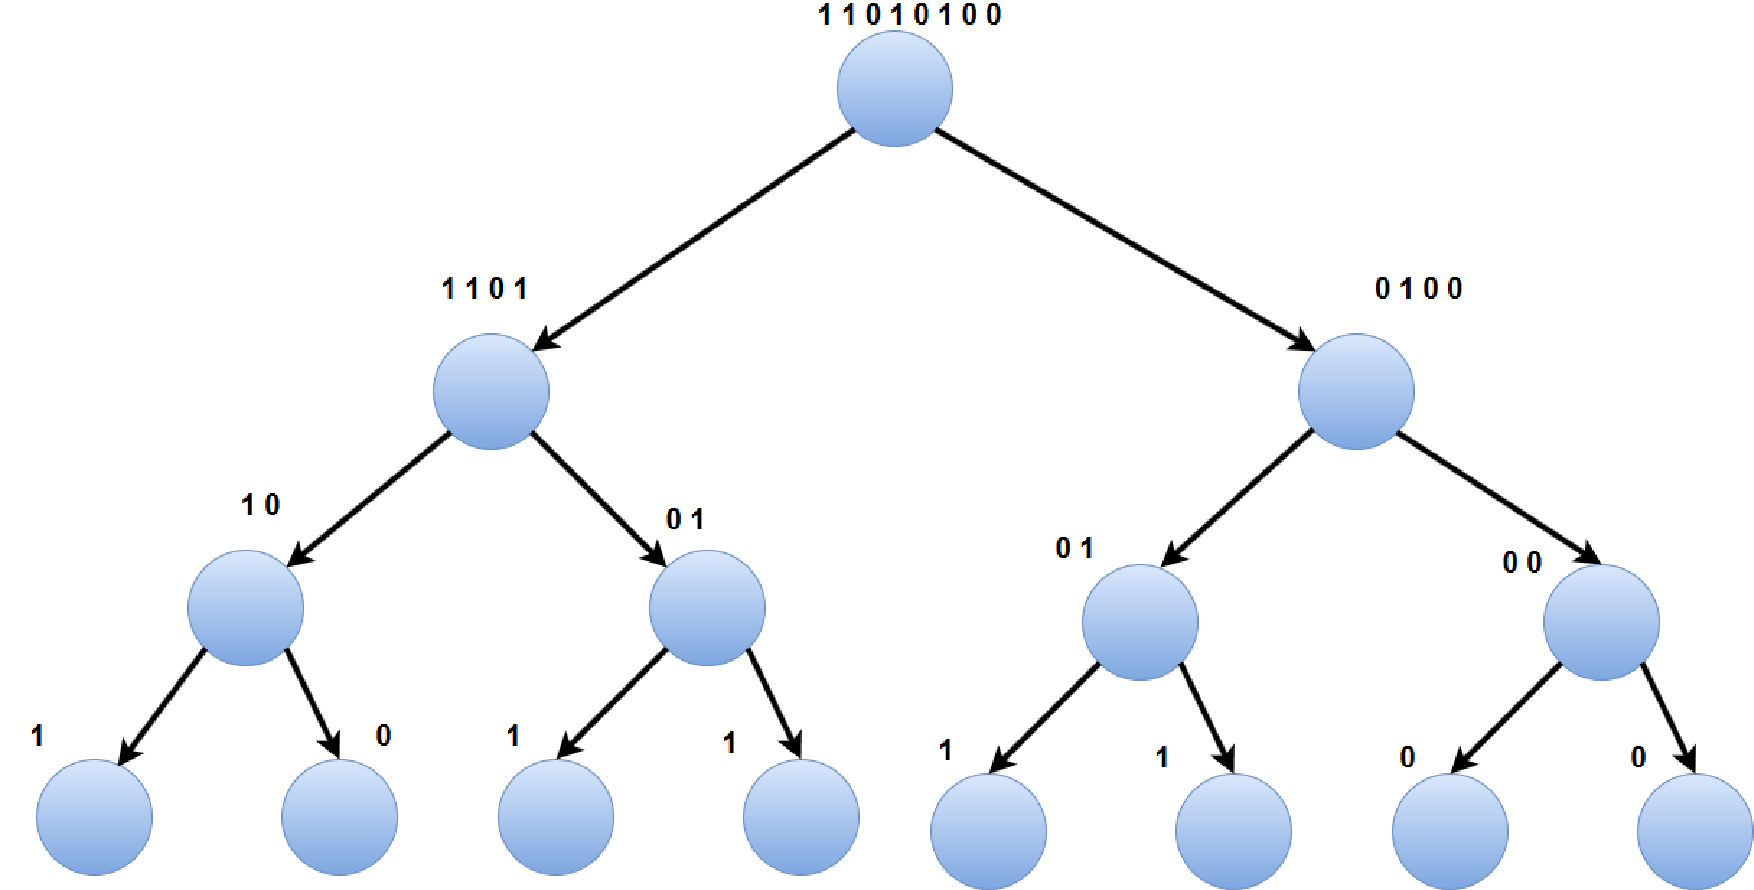
\includegraphics[width=0.7\textwidth]{./figures/treeEncoding.pdf}
	\caption{Encoding tree}
	\label{fig:treeEncoding}
\end{figure}

As it can be observed from the tree, same operation is performed at every node only the size of a vector is different, due to the regular structure encoding problem fits the recursive algorithmic form. Algorithm in ~\ref{algo:polarEncoder} shows a naive implementation of recursive encoder. In the algorithm shown in ~\ref{algo:polarEncoder} each bit is represented a one integer, hence each bit is processed serially parallelism is not exploited. Upon profiling the implementation it also identified that ~\ref{line:copying1} and ~\ref{line:copying2} are also the bottlenecks since copying is involved. One more issue with the algorithm in ~\ref{algo:polarEncoder} is the recursive implementation. Although the encoding can be easily implemented with this algorithm, each recursive function call in software is expensive, since it requires a new stack frame to be allocated each time.

\IncMargin{1.5em}
\begin{algorithm}[]
	\KwData{$u_{\textit{0}}^{\textit{N-1}}$,$N$,$dIndex = 0$}
	\KwResult{$y_{\textit{0}}^{\textit{N-1}}$}
	\SetKwFunction{FMain}{recursiveEncode}
	\SetKwProg{Fn}{function}{:}{}
	\Fn{\FMain{$u_{\textit{0}}^{\textit{l-1}}$,$l$}}{
		\If {$l == 1$} {
			$y_{dIndex} = u_{0}$ \;
			$dIndex = dIndex + 1$ \;
		} \Else {
			$len = \frac{l}{2}$ \;
			$P_{\textit{0}}^{\textit{len-1}}$ = $u_{\textit{0}}^{\textit{len-1}}$ \; 	\label{line:copying1}
			$Q_{\textit{0}}^{\textit{len-1}} = u_{\textit{len}}^{\textit{l-1}}$ \;		\label{line:copying2}
			
			\For{$i=0$ to $length-1$} {													\label{line:xor1}
				$P_{\textit{i}} = P_{\textit{i}} \oplus Q_{\textit{i}}$\;				\label{line:xor2}
			}
			
			\FMain{$P_{\textit{0}}^{\textit{len-1}}$,$len$} \;
			\FMain{$Q_{\textit{0}}^{\textit{len-1}}$,$len$}	\;
		}
	}
	\caption{Naive polar encoder}
	\label{algo:polarEncoder}	
\end{algorithm}
\DecMargin{1.5em}

To avoid the disadvantages mentioned above, following optimization techniques are considered.

$\bullet$ \textbf{Parallel processing:} To avoid the serial processing of bits and for improving the parallelism factor, method described in section ~\ref{dataPackUnpack} is used, i.e is multiple bits are packed to single integer, in this particular instance, every 64 bits of are packed into 64-bit integers so that 64-bits can be processed in parallel with 64-bit supported processor, which results in a parallelism factor ($\mathcal{P}$) of 64. Packing also helps to further increase the parallelism factor $\mathcal{P}$ with state of the art SIMD processing units of the modern processors. SIMD instructions can process of 256-bit or 128-bit in a single instruction which results in a parallelism factor ($\mathcal{P}$) of 256 with AVX and 128 with SSE instructions. \newline
\newline
$\bullet$ \textbf{Avoiding the copy operations:} Naive algorithm in ~\ref{algo:polarEncoder} splits the of $N$-bits into two $\frac{N}{2}$-bit vectors and copies them temporarily allocated variables. Code profiling pointed out that these copying operations are the bottlenecks. In optimized algorithm, instead of copying, C++ pointers concept is used to calculate the index where next block of vector starts and this index is passed to next node for further processing. \newline
\newline
$\bullet$ \textbf{Unrolling the encoder:} Recursive implementation has significant overhead due to the huge number of recursive function calls which require new stack frame allocation. To avoid this overhead, encoder implementation is unrolled, in other words, new inline functions are defined for each vector size. Advantages of these functions is that they don't won't require new stack frame to be allocated when an inline function is called, they will make use of stack frame from which they are called. However this requires a separate inline function for every vector size. Having a different function for every vector size also has advantages, which allows us to use SIMD instructions whenever vector size can fit SIMD registers otherwise normal instructions can be used. \newline
\newline
$\bullet$ \textbf{Pruning encoder tree:} As shown in the figure ~\ref{fig:treeEncoding}, encoding process can be represented as traversal of a binary tree. When an encoding is implemented in software, when traversing the tree towards leaf nodes, bit vector size can becomes less than 8 bits, which requires accessing 4/2/1 bits of an integer. In standard processors smallest unit which can be accessed is an 8-bit integer. To access 4/2/1 bits masking operations are needed. Since the nodes in a binary tree which access 4,2,1 bits is huge, significant number of masking operations are needed, which introduces a added overhead. Pruning of tree at level where the bit vector size is 8, avoids this overhead in addition to reducing the number of nodes to be traversed in a binary tree. Pruning is done by building a lookup table containing encoded value for every combination of 8-bit vector and reading the value from lookup table for the encoded value when the bit vector size is 8. Lookup table will contain 256 bytes, containing encoded value for every combination of 8-bit vector.\newline
\newline
Pruning of the tree had a significant latency improvement, it can be better understood by taking an example. In a scenario where $N = 1024$, with unpruned tree number of nodes to be traversed for encoding is 2047 nodes, out of these nodes contain 1024 1-bit, 512 2-bit and 256 4-bit nodes. With pruned tree 4/2/1 bit nodes are not present, number of nodes to be traversed reduces to 255 from 2047. Pruning avoids masking operations as well as tree traversal. \newline
\newline
Example of a pruned unrolled encoder containing also the tree traversal is shown in the figure ~\ref{fig:unrolledEncoder}. Inline function names for different bit vector size are also shown in the figure. One can see that tree traversing ends at $bitMult8$ function due to pruning. Tree traversal flow is represented with orange line in a figure.

Sample code snippet of node operation with SIMD instructions is shown in a listing ~\ref{code:simdNodeOps}.

\begin{table}[]
	\begin{center}
		\caption{Latency comparison: polar encoding for 1024 bits}
		\label{tab:polarEncoder}
		\begin{tabular}{c|c|c} % <-- Alignments: 1st column left, 2nd middle and 3rd right, with vertical lines in between
			\textbf{ } & Naive & Optimized \\
			\hline
			Latency ($\mu$s) & $34$ & $0.244$\\
		\end{tabular}
	\end{center}
\end{table}

\begin{figure}[]
	\centering
	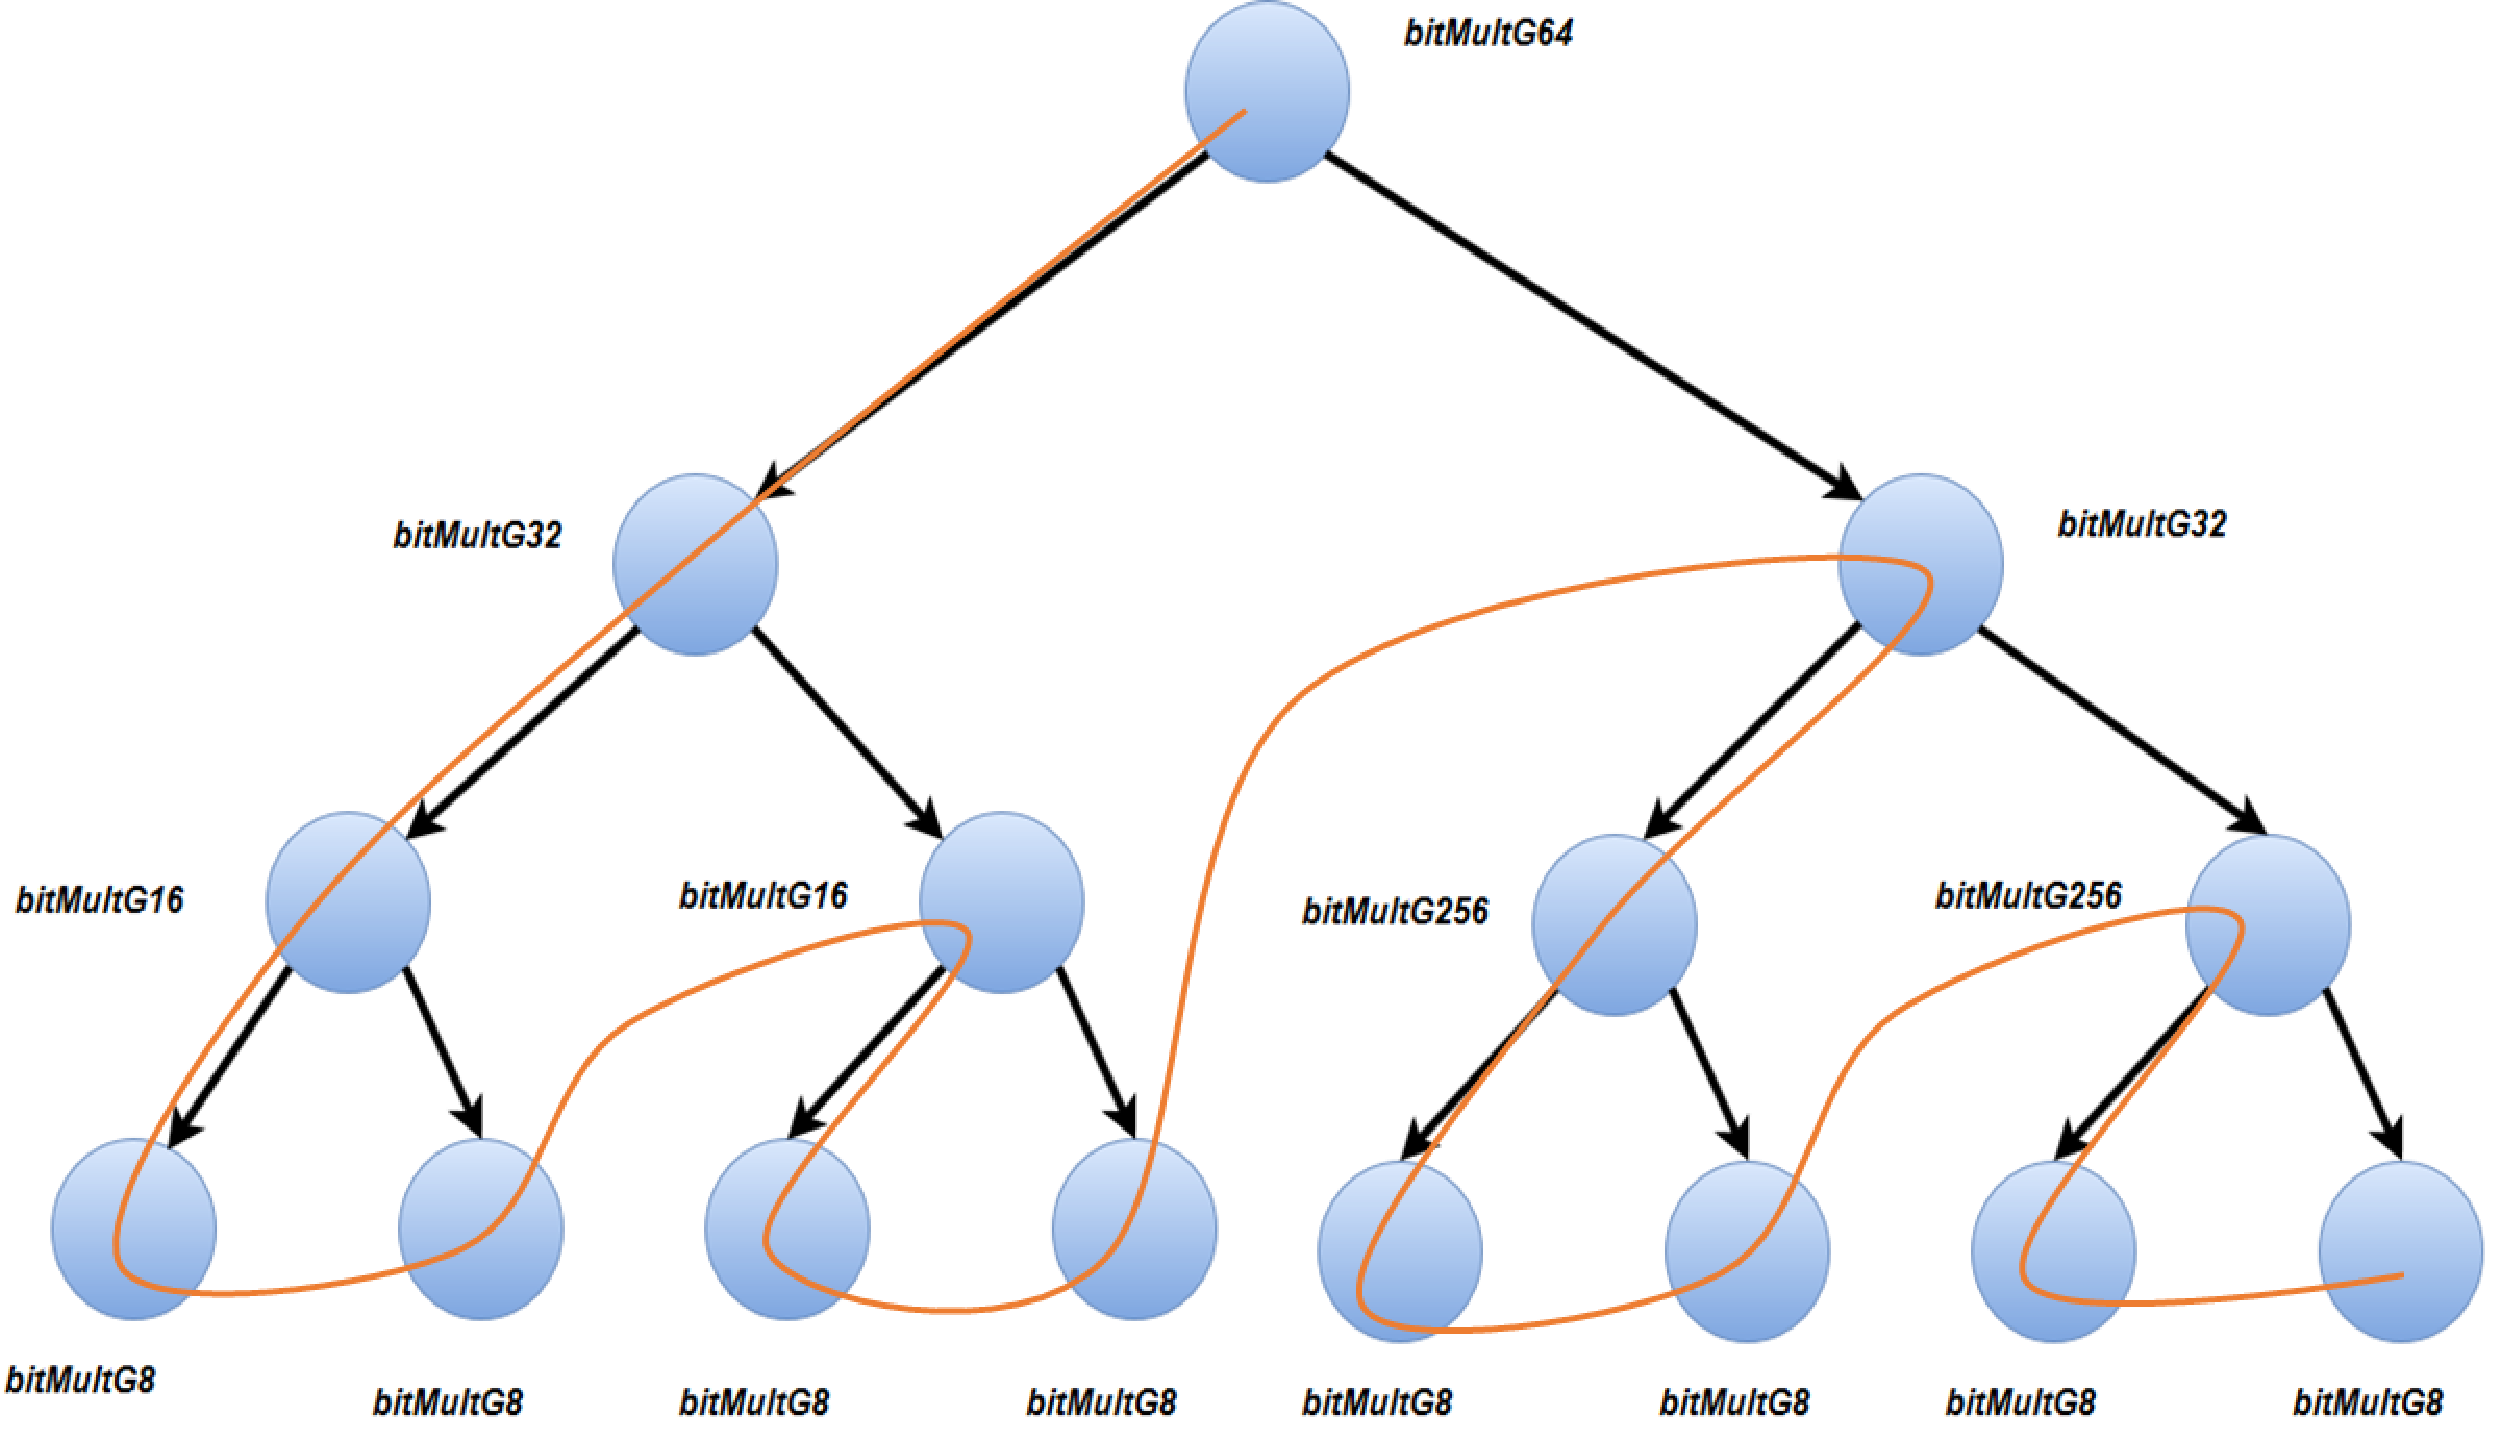
\includegraphics[width=0.7\textwidth]{./figures/unrolledEncoder.pdf}
	\caption{Pruned unrolled encoder tree}
	\label{fig:unrolledEncoder}
\end{figure}

\begin{lstlisting}
inline void bitMultG512(uint8_t *s, uint8_t *dEncoded) 
{
  //Here s is 64 bytes, Divided to 32 bytes each.
  uint8_t *s1 = (uint8_t *) s;
  uint8_t *s2 = (uint8_t *) (s + 32);
  __m256i result;
  __m256i temp1 = _mm256_loadu_si256((__m256i*)operand1);
  __m256i temp2 = _mm256_loadu_si256((__m256i*)operand2);
  result = _mm256_xor_si256(temp1,temp2);
  _mm256_storeu_si256((__m256i*)destn, result);
  bitMultG256((uint8_t *) s1, dEncoded);
  bitMultG256((uint8_t *) s2, dEncoded);
}
\caption{SIMD implementation of node operation in a encoder tree}
\label{code:simdNodeOps}
\end{lstlisting}

\section{Rate matching}

\section{Results Comparison}



 % Contains the details of encoding FEC chain.
        %%%%%%%%%%%%%%%%%%%%%%%%%%%%%%%%%%%%%%%%%%%%%%%
\chapter{Decoding FEC Chain} \label{chap:DecodingChain}
%%%%%%%%%%%%%%%%%%%%%%%%%%%%%%%%%%%%%%%%%%%%%%%
In this chapter, implementation and optimization details of 5G polar decoding FEC are presented including challenges faced while achieving low latency decoding. In the FEC chain, decoder is the critical part due to inherent sequential nature of polar decoding. $n^{th}$ bit is decoded by using all the previously decoded bits, hence $n^{th}$ bit depends on $0$ to $n-1$ bits. Due to sequential decoding process, significant latency is introduced by the decoder. This section presents the optimization techniques employed to improve decoding FEC chain latency, which include both algorithmic and platform specific optimizations. Each these techniques are explained in the respective sections where these are employed. In this work, FEC chain considered is part of the base station, therefore uplink control information is decoded at receiver. PUCCH (Physical uplink control channel) and PUSCH (Physical uplink shared channel) contain polar encoded information. Received signal after demodulation is quantized to 16-bit LLR (log likelihood ratio) values. Decoding is performed with LLR (Log likelihood ratio) values rather than probabilistic likelihoods due to their numerical stability and low computational complexity. Receiver side FEC chain is a reverse of the operations performed at transmitter. Figure ~\ref{fig:5grx_fec_chain} shows the receiver side polar decoding FEC chain.

\begin{figure}[]
	\centering
	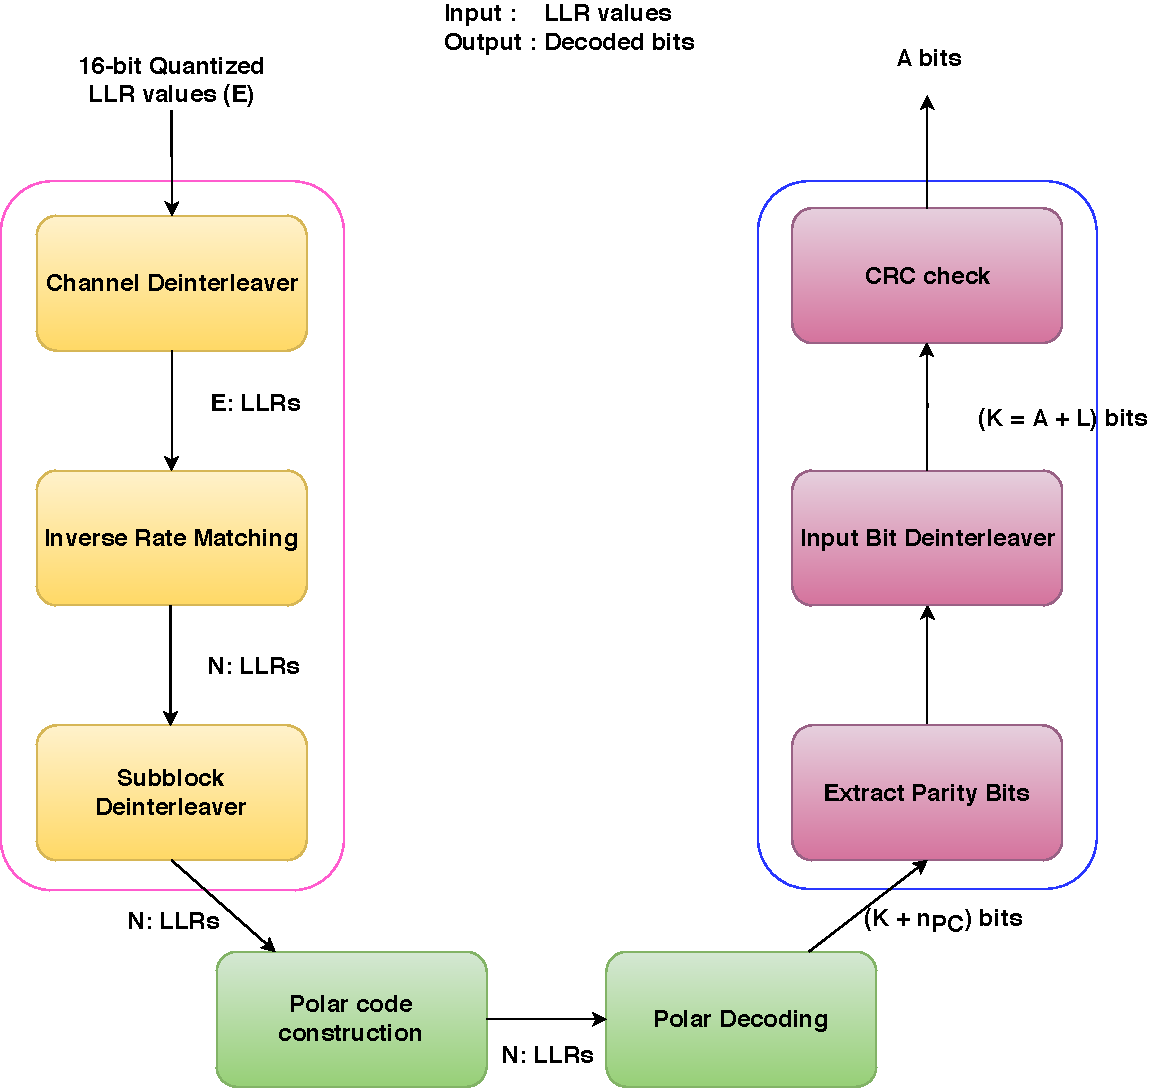
\includegraphics[width=0.7\textwidth]{./figures/receiverFECChain_crc.pdf}
	\caption{Polar decoding FEC chain for PUCCH/PUSCH}
	\label{fig:5grx_fec_chain}
\end{figure}

%$\mathtt{Yadhu}$
%\NOTE{Decoding is of serial nature, has lot of latency. Polar decoding chain necessity. PUCCH and PUSCH, parameters of both the channels.}
%%	Explain all the decoding Optimizations I have done, In this document.
%% 	Explain of the latency without optimization.

\section{Decoding algorithms}
The basic decoding algorithm successive cancellation (SC) is developed by the Arikan in his seminal work on polar codes \cite{Arikan}. It achieves the symmetrical capacity of binary memoryless channel through sequential decoding when block length is very large. However due to the sequential nature significant latency is introduced by decoding algorithm. Latest 5G standard specifies transmission time interval (TTI) of $125 \mu s$ \TODO{cite the doc}, within this duration scheduling and encoding/decoding must be done. Therefore it is very important to efficiently perform FEC chain operations. This work concentrates on implementing the polar encoding/decoding in software and studies the feasibility of satisfying the strict latency requirements of 5G. Decoding through SC algorithm can be represented as binary tree, decoding process is nothing but traversing through a tree sequentially. Significant research work is done both in academia and industry to improve decoding latency of the SC algorithm. Major improvement to SC which significantly reduced the decoding latency is identifying special kind nodes in a tree which allow immediate decoding of multiple bits without requiring full tree traversal. Algorithms presented in \cite{SSC} and \cite{fastSSC} present such improvements, which identify special nodes or in other words component codes such as \textit{Rate-0}, \textit{Rate-1}, \textit{RPC} and \textit{SPC} nodes, \textit{RPC} and \textit{SPC} mean repetition and single parity check code respectively. Identification of special nodes requires finding particular patterns the frozen bit locations in the constructed polar code. To gain full advantages of Fast-SSC (Fast Simplified Successive Cancellation) algorithm, special nodes must be identified efficiently. In this work, 5G RX FEC chain with fast-SSC algorithm implemented/optimized in software and feasibility of achieving desired latency( $< 50\mu s$) is analyzed.
%Following sections present how processor specific features are exploited to efficiently identify


\section{Decoding chain}
The figure ~\ref{fig:5grx_fec_chain} shows the complete receiver side FEC chain. It is almost a inverse operations of encoding FEC chain except few differences related to PUCCH and PDSCH which contain parity check bits ($ n_{PC} $). The decoding FEC chain receives UCI(Uplink Control Information) in the form of 16-bit quantized $ E $ LLR values. Before passing LLR values to decoder inverse operations of the steps which were carried out aftermath of encoding, which are channel deinterleaving, inverse rate matching and subblock deinterleaving. These steps grouped by a pink rectangle in the figure, after these steps polar code construction is performed using same optimized method as presented in the previous chapter. Polar code construction procedure outputs the information bit positions, from which frozen pattern can be obtained. Next step in the FEC chain is polar decoding, $ N $ LLR values and frozen pattern is passed to polar decoder, which outputs the decoded bits. Polar construction and decoding blocks are colored green the FEC chain figure. Using information bit positions obtained in the polar construction procedure $ K + n_{PC} + L $ bits are extracted from $ N $ decoded bits. $ K + n_{PC} + L $ bits contain $ n_{PC} $ parity bits, extracting these bits requires identifying the row of minimum weight from the generator matrix of polar code. Finally input deinterleaving is applied on the remaining $ K +  L $ bits to obtain concatenated information and CRC bits. Blocks representing Extracting parity bits and input bit deinterleaver are grouped with blue rectangle. In this section, we presented briefly the functionalities carried out by different blocks of the decoding FEC chain. Next we will analyze the latency contributions of each those operations and come up with optimizations both algorithmic and platform specific to reduce latency.

\section{Channel deinterlever}
The first operation after receiving the LLR values is channel deinterleaving, This is the exact inverse of the interleaving operation done at the transmitter. Channel interleaving is performed to make transmission robust against burst errors. Authors of \cite{3gpp.TSG-RAN_WG1} analyze the error correction performance of polar codes for different channel conditions and constellations. It is found that error correction performance significantly deteriorates for constellations 16-QAM onwards. Channel interleaving wasn't done for downlink PBCH/PDCCH since the constellation was QPSK, however in case of PUCCH/PUSCH higher constellations are used hence channel interleaving is necessary. In 5G standard  isosceles right triangle interleaver is adopted. Deinterleaving is carried out by writing LLR values to columns of triangular structure and reading LLR values in rows. Interleaver design is proposed by Qualcomm \cite{3gpp.TSG-RAN_WG1}.

Vector processing instructions cannot be used for the implementation of interleaver due irregular and non uniform memory access, therefore interleaver just plain functional implementation. One optimization technique was to avoid new memory allocation and using already allocated memory. This avoids the overhead of dynamic memory allocation and initialization. Channel deinterleaving is one of significant contributor to latency in polar decoding FEC chain, since each of the LLR values need to processed sequentially.

\section{Inverse rate matching}
Inverse rate matching step maps the $E$ LLR values to mother code block size $ N $. Rate matching step has three modes puncturing, shortening and repetition. Mode is selected based on rate matcher output size ($E$) and mother code size($ N $). If $E > N$ then repetition performed, otherwise either puncturing and shortening is done. If $ \frac{K}{E} > \frac{7}{16} $ shortening else puncturing is performed. Major optimization in inverse rate matching are utilizing SIMD capability for soft combining when $ E>N $ and performing block wise copying. \NOTE{Does it makes sense to explain criteria why and when puncturing or shortening is selected}
%
%to and avoiding a copying operations when the mode is shortening or puncturing instead using a pointer manipulation to select
%Software optimization in inverse rate matching is performed by Empirically it is observed that shi  type of rate matching is selected based on code rate.
%
\section{Sub-block de-interleaver}
After inverse rate matching, $E$ values are mapped to $N$ LLRs, which is always a power of two. Subblock interleaver/deinterlever divides block of $N$ LLRs into $32$ subblocks, each containing $\frac{N}{32}$ LLRs. Functionally, subblock deinterleaving can be implemented as a inverse of interleaving operation as presented in \cite{3gpp.38.212}. Upon measuring the latency contribution of subblock deinterleaver it was found to be taking $10 \mu s$. Computation complexity of interleaving indexes huge due to the use of multiplication, division and modulus operations. \newline

\begin{figure}[]
	\centering
	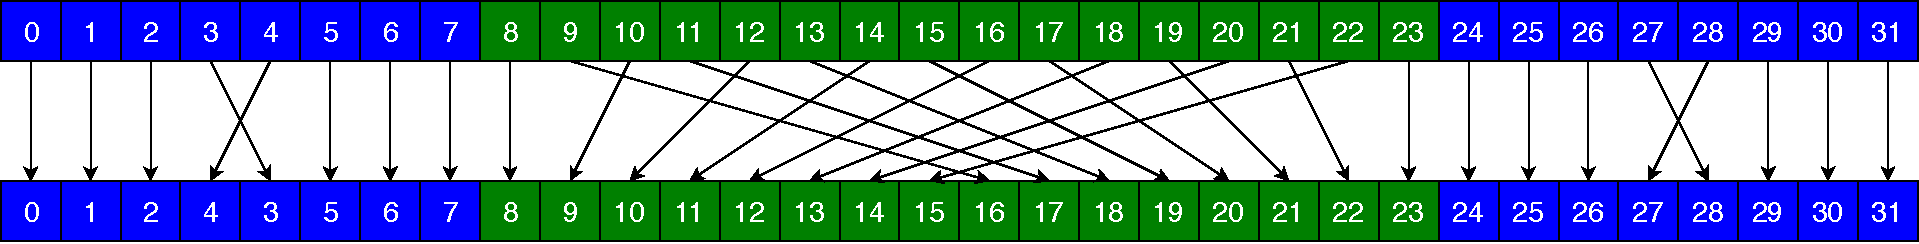
\includegraphics[width=1.0\textwidth]{./figures/subblockDeinterleaver.pdf}
	\caption{Subblock deinterleaving pattern}
	\label{fig:subblockDeinterleaver}
\end{figure}

If we look at the figure ~\ref{fig:subblockDeinterleaver}, we can see that not all the values of LLRs are interleaved, only 18 positions out of 32. Calculating interleaving positions is expensive instead they can be pre-calculated and stored in a lookup table. For the mother code size of 1024, with pre-calculated positions interleaving requires looping for $ 576 $ times. Modern processors with \textit{AVX} and \textit{AVX2} extensions provide special swizzle instructions, which allow shuffling, permuting and blending of vectors. These instructions process vector of values hence allow data parallelism. To make use of swizzle instructions for subblock deinterleaving, it must be reformulated to fit into functionality provided by platform specific SIMD instructions. It is divided into three parts, each one is independent of another. Part one and three are exactly same operations each dealing with 8 subblocks and performing the operation marked by green in the figure. Part one and three are mapped to shuffle SIMD instructions. Part two deals with 16 subblocks, marked by blue in the figure. Part two operation is achieved with blend and permute SIMD instructions.

Code snippet in the listing ~\ref{code:subblockDeinterleaver} shows sample SIMD implementation of subblock deinterleaving operation for mother code size ($N$) 64.

\begin{code}
\captionof{listing}{Vectorized Subblock deinterleaving for $N = 64$}
\label{code:subblockDeinterleaver}
\begin{minted}{c++}
void subblockdeinterleaver64( int16_t y[], int16_t d[]) {
	__m256i v256_in,v256_perm0,v256_out,v256_perm1,v256_perm2;
	__m256i v256_out2,v256_blended,v256_perm3;
	//interleaving pattern, precalculated is encoded here.
	v256_perm0 = _mm256_setr_epi32(0,1,2,4,3,5,6,7);
	v256_perm1 = _mm256_setr_epi32(0,2,4,6,1,3,5,7);
	v256_perm2 = _mm256_setr_epi32(1,3,5,7,0,2,4,6);
	v256_perm3 = _mm256_setr_epi32(4,5,6,7,0,1,2,3);
	//prepare part1
	v256_in = _mm256_loadu_si256((__m256i*)y);
	v256_out = _mm256_permutevar8x32_epi32 (v256_in,v256_perm0);
	_mm256_storeu_si256((__m256i*)d,v256_out);
	//prepare part2
	v256_in = _mm256_loadu_si256((__m256i*)(y + 16));
	v256_out = _mm256_permutevar8x32_epi32 (v256_in,v256_perm1);
	v256_in = _mm256_loadu_si256((__m256i*)(y + 32));
	v256_out2 = _mm256_permutevar8x32_epi32(v256_in,v256_perm2);
	v256_blended = _mm256_blend_epi32 (v256_out,v256_out2,0b11110000);
	_mm256_storeu_si256((__m256i*)(d  + 16),v256_blended);
	v256_out2 = _mm256_permutevar8x32_epi32(v256_out, v256_perm3);
	v256_out = _mm256_permutevar8x32_epi32(v256_in, v256_perm1);
	v256_blended = _mm256_blend_epi32(v256_out2,v256_out,0b11110000);
	_mm256_storeu_si256((__m256i*)(d + 32),v256_blended);
	//prepare part3, same as part1
	v256_in = _mm256_loadu_si256((__m256i*)(y + 48));
	v256_out = _mm256_permutevar8x32_epi32 (v256_in,v256_perm0);
	_mm256_storeu_si256((__m256i*)(d + 48),v256_out);
		
}
\end{minted}
\end{code}

Results Latency optimization of subblock deinterleaver for $N = 1024$ is given the table ~\ref{tab:subblockDeinterleaverLatency}.
\begin{table}[!h]
	\begin{center}
		\caption{Latency comparison: Subblock deinterleaver}
		\label{tab:subblockDeinterleaverLatency}
		\begin{tabular}{c|c|c} % <-- Alignments: 1st column left, 2nd middle and 3rd right, with vertical lines in between
			\textbf{ } & Naive & Optimized \\
			\hline
			Latency ($\mu$s) & $19.7$ & $0.47$\\
		\end{tabular}
	\end{center}
\end{table}

\section{Decoder optimization}
This section discusses the details of decoder implementation and optimizations. Fast-SSC algorithm is considered due low complexity and ability to parallelize the decoding operations. Fast-SSC is an improved version basic SC algorithm. It identifies the special nodes which can be decoded without traversing the full tree. Special nodes are decoded efficiently using SIMD instructions which further reduces the decoding latency. Many software optimizations are performed. Each of them discussed in this section.

\subsection{VN and CN operations}
Polar decoding with Fast-SSC algorithm is equivalent to traversing binary tree. Every node in a tree involves one pair CN and VN operations. Result of CN operation is passed to left child and VN operation result to the right child. Number of nodes in a tree are exponential dependent on the block-length of a code. For block length of 1024 number nodes in a binary tree are 2047. Decoding requires 2047, CN and VN operations, hence it is very critical to implement CN and VN operations efficiently. In this work LLR's are quantized to 16-bit integers hence decoder is a 16-bit fixed point implementation. At each node, vector of LLRs is received from the parent node. CN and VN operations are performed on the received vector.

\begin{code}
\captionof{listing}{Vectorized CN operation}
\label{code:CnOperartion}
\begin{minted}{c++}
template<unsigned int NvDash>
void CnOp(int16_t alphaL[],int16_t demodLLRs[]) {
  __m256i temp1,temp2,mag_temp1,mag_temp2;
  _m_prefetch(alphaL);
  _m_prefetch(demodLLRs);
  for(unsigned i = 0; i < NvDash; i = i + 16) {
	temp1 = _mm256_loadu_si256((__m256i*)(demodLLRs + i));
	temp2 = _mm256_loadu_si256((__m256i*)(demodLLRs + NvDash + i));
	mag_temp1 = _mm256_abs_epi16 (temp1);
	mag_temp2 = _mm256_abs_epi16 (temp2);
	mag_temp1 = _mm256_min_epi16 (mag_temp1, mag_temp2);
	temp1 = _mm256_sign_epi16(temp1, temp2);
	temp1 = _mm256_sign_epi16(mag_temp1, temp1);
	_mm256_storeu_si256((__m256i*)(alphaL + i),temp1);
  }
}
\end{minted}
\end{code}
\begin{code}
\captionof{listing}{Vectorized VN operation}
\label{code:VnOperartion}
\begin{minted}{c++}
template<unsigned int NvDash>
void VnOp(int16_t alphaR[],int16_t demodLLRs[],int8_t betaL[]) {
  __m256i alphaLeft,alphaRight,beta;
  _m_prefetch(alphaR);
  _m_prefetch(demodLLRs);
  for(unsigned i = 0; i < NvDash; i = i + 16) {
    alphaLeft = _mm256_loadu_si256((__m256i*)(demodLLRs + i));
    alphaRight = _mm256_loadu_si256((__m256i*)(demodLLRs + i + NvDash));
    beta = _mm256_cvtepu8_epi16(_mm_loadu_si128((__m128i*)(betaL + i)));
    beta  = _mm256_slli_epi16(beta,15);
    beta = _mm256_or_si256(beta,_mm256_set1_epi16(1));
    alphaLeft = _mm256_sign_epi16(alphaLeft,beta);
    alphaRight = _mm256_add_epi16(alphaRight,alphaLeft);
    _mm256_storeu_si256((__m256i*)(alphaR + i),alphaRight);
  }
}
\end{minted}
\end{code}
If CN operation needs to performed on received vector, naive method would be to access each value from the vector to perform the same CN operation. Sequentially performing CN and VN operations is very inefficient. Size of the vector received at each node is always a power of 2. Due to this fact CN and VN operations naturally fit vector processing units provided in the modern processors. In this work both CN and VN operations are efficiently implemented using SSE and AVX instruction extensions provided by AMD APYC platform. During CN and VN operations memory access is regular therefore data required in the future can be fetched to cache from main memory to reduce cache misses. Listing given in \ref{code:CnOperartion} and \ref{code:VnOperartion} show the efficient vectorized CN and VN operations.


\subsection{Identifying component codes}
%How different kind of sub code types are identified efficiently using with bit packed frozen bits.
As explained in the beginning of this chapter, naive SC algorithm purely sequential, hence decoder introduces significant latency in the FEC chain. With improvements such as \cite{fastSSC} and \cite{SSC} decoding tree can be pruned by identifying particular patterns in frozen bit positions. Pruning of a tree allows decoding multiple bits in parallel. Component codes out of polar codes can be identified which allow decoding without traversing the full decoder tree. Authors in \cite{SSC} and \cite{fastSSC} identify four such codes namely rate-0, rate-1, repetition and single parity codes. Decoding a code word through component codes improves latency without compromising the error correction performance. However to fully enjoy the fruits decoding tree pruning, implementation should be able identify component codes efficiently. One simple functional way is to go through all frozen bits and search by comparing with predefined patterns. Naive way of searching for a pattern introduces significant latency in the decoding process. Processors with \textit{AVX} and \textit{AVX2} support contain registers which can store 256/128 bits in a single register. Frozen pattern array/vector contain either one or zero, one indicating frozen bit and zero information bit. Since one bit is enough to represent type of bit position, frozen pattern can be stored by packing multiple bits type information to single 256bit register which allows identifying a pattern by comparing with a integer using single SIMD instruction. As an example with a mother code size $N=256$ information about which position is frozen and which is not can stored in a single 256 bit SIMD register in a bit packed format. To check whether it is a rate-0, rate-1, SPC or RPC requires one SIMD comparison instruction. Snippet in a listing ~\ref{code:rateZeroSIMDComparison} illustrates an example of identifying node type in bitpacked frozen bits pattern.
\begin{code}
	\captionof{listing}{Checking rate-0 node}
	\label{code:rateZeroSIMDComparison}
	\begin{minted}{c++}
template<>
inline int identify_R0<256>(uint64_t s[]) {
	__m256i temp1 = _mm256_loadu_si256 ((__m256i*)s);
	__m256i temp2;
	temp2 = _mm256_set1_epi8 ((char)0xFF);
	__m256i pcmp = _mm256_cmpeq_epi64 (temp1, temp2);
	unsigned bitmask = _mm256_movemask_epi8(pcmp);
	return (bitmask == 0xffffffffU);
}
\end{minted}
\end{code}

\subsection{Decoding Rate-0 code}
Rate-0 code is a special kind of node in a decoding tree in which all the descendants represent frozen bit positions, in other words corresponding node's frozen pattern contains all ones. One such example is given in the background section. For such a node, we know that all the bits are frozen hence decoder can immediately decode values as zero. All the decoded bits corresponding to such a node are set to zero. Rate-0 node allows decoder to avoid performing VN and CN operations at the subsequent child nodes in addition to decoding multiple bits simultaneously.

\subsection{Decoding Rate-1 code}
A node is considered as Rate-1 node, if all of its descendants in a decoder tree are information bits. In other words the Rate one node contains no frozen bits. Decoding of Rate-one can also be performed without traversing till the end of a decoder and hence avoiding significant number of VN and CN operation. However decoding Rate-1 node is not as straight forward as Rate-0 node. Decoding is done through threshold detection of all the LLRs and performing polar transform on the result to obtain decoded bits.

\IncMargin{1.5em}
\begin{algorithm}[]
	\KwData{$\alpha_{v}^{N_v-1}$, $N_v$}
	\KwResult{$y_{0}^{N_v-1}$, $\beta_{0}^{N_v-1}$}
	\SetKwFunction{FMain}{decodeR1}
	\SetKwProg{Fn}{function}{:}{}
	\Fn{\FMain{$\alpha_{v}^{N_v-1}$,$y_{0}^{N_v-1}$, $\beta_{0}^{N_v-1}$}} {
		\For{$i=0$ to $N_v-1$} {
			$\beta_{v}[i] = \alpha_{v}[i] \ge 0$\;
		}
		$y_{0}^{N_v-1} = polarTransform(\beta_{0}^{N_v-1})$ \;
	}
	\caption{Rate-1 node decoding algorithm}
	\label{algo:R1Decoding}
\end{algorithm}
\DecMargin{1.5em}

Although Rate-1 nodes avoids CN and VN operations, decoding is not parallel. Decoder needs to go through each of the LLRs to decode the bits and finally perform polar transform. Both of which are costly operations. To improve the latency through data parallelism, threshold detection can make use of SIMD instructions. Threshold detection of a complete vector can be performed through single SIMD comparison instruction.This improves the parallelism factor to sixteen for 16-bit LLRs with {AVX2} instructions. The code snippet in listing ~\ref{code:rateOneNodeDecoding} presents an example where rate-1 node decoding is implemented using AVX instructions. Resulting in parallelism factor is eight.

\begin{code}
	\captionof{listing}{Decoding rate-1 subcode}
	\label{code:rateOneNodeDecoding}
	\begin{minted}{c++}
template<unsigned Nv>
void decR_1(int16_t demodLLRs[],int8_t beta[],int8_t decodedBits[]) {
  __m128i temp1,tempDecodedVec;
  _m_prefetch(beta);
  _m_prefetch(decodedBits);
  for(unsigned i = 0; i < Nv; i = i + 8) {
    temp1 = _mm_loadu_si128((__m128i*)(demodLLRs + i));
    tempDecodedVec = _mm_cmplt_epi16(temp1,zeros);
    tempDecodedVec = tempDecodedVec & _mm_set1_epi16(1);
    tempDecodedVec = _mm_packs_epi16(tempDecodedVec,_mm_setzero_si128());
    _mm_storeu_si128((__m128i*)(beta + i),tempDecodedVec);
    _mm_storeu_si128((__m128i*)(decodedBits + i),tempDecodedVec);
  }
  polarTransform<Nv>(decodedBits,decodedBits);
}
\end{minted}
\end{code}

Next step in decoding rate-1 node is performing polar transform operation. It is equivalent to performing polar encoding. As explained in the previous chapter, binary tree represents encoding process. Efficient polar transform implementation makes use of same optimizations techniques employed in encoder such as SIMD vectorization and look up table techniques.

\subsection{Decoding RPC code}
Repetition code (RPC) is another type of sub code which be identified from polar code. It allows decoding multiple bits without tree full tree traversal. A node is considered as RPC when only one its right most descendent contains information and all remaining bits are frozen. Bit packed frozen pattern allows easy identification of RPC node. If frozen pattern at the node is equal to one then it is a RPC node. RPC node decoding is similar to simple repetition code decoding by adding all the LLRs and doing threshold detection for the sum.  Result of threshold detection is stored at information bit position and remaining bits at the node are set to zero.

\begin{equation*}
 \beta_{v}[i] = \begin{cases}
				0, \text{ when $\sum_{j} \alpha_{v}[j] \geq 0 ;$}  \\
				1, \text{ otherwise.}
				\end{cases}
\end{equation*}

Again, RPC-node decoding process has scope for improvement. Decoding requires summing of all LLRs. Summation operation efficiently performed with SIMD instructions through data parallelism instead of adding individual values. This vectorization has significant gain when sum of huge LLR vector is required.

\subsection{Decoding SPC code}
Another type of constituent codes which can be decoded more efficiently without complete tree traversal is single-parity check (SPC) code. These nodes have a code rate $Nv-1/Nv$. In other words, these nodes have only one frozen bit at right most position. Optimal ML decoding of SPC codes can be performed in an optimal way with very low complexity. Similar to Rate-1 code decoding SPC code requires threshold detection for all the LLRs. To achieve this efficiently same optimizations employed to Rate-1 code are reused. For SPC decoding two more additional steps are required namely finding position of minimum magnitude LLR and calculating the parity of decoded bits. If the parity of decoded bits is not even then bit value at the position of lowest magnitude LLR is flipped. Final step in the decoding is to obtain final decoded bits values through polar transform. The steps described above are shown in the algorithm ~\ref{algo:spcDecoding}.

\IncMargin{1.5em}
\begin{algorithm}[]
	\KwData{$\alpha_{v}^{N_v-1}$, $N_v$}
	\KwResult{$y_{0}^{N_v-1}$, $\beta_{0}^{N_v-1}$}
	\SetKwFunction{FMain}{decodeSpc}
	\SetKwProg{Fn}{function}{:}{}
	\Fn{\FMain{$\alpha_{v}^{N_v-1}$,$y_{0}^{N_v-1}$, $\beta_{0}^{N_v-1}$}} {
			$j = \alpha_{v}[i]$ \;
			$parity = 0$ \;
			\For{$i=0$ to $N_v-1$} {
				$\beta_{v}[i] = \alpha_{v}[i] \ge 0$\;
				\If {$j < |\alpha_{v}[i]|$} {
					$j = i$ \;
				}
				$parity = parity + \beta_{\textit{i}}[i]$ \;
			}
		\If {$parity \neq 0$} {
			$\beta_{v}[j] = 1 - \beta_{v}[j]$\;
		}
		$y_{0}^{N_v-1} = polarTransform(\beta_{0}^{N_v-1})$ \;
		}
	\caption{SPC decoding}
	\label{algo:spcDecoding}
\end{algorithm}
\DecMargin{1.5em}

SPC code uses same two operations (threshold detection and polar transform) as used in RPC decoding. This allows reusing of same optimization techniques. Two additional operations in SPC decoding are finding the position of minimum magnitude LLR and calculating the parity. Time complexity of finding a minimum magnitude LLR position is $\mathcal{O}\big(N\big)$. It can be reduced to $\mathcal{O}\big(N/8\big)$ by mapping search operation to SIMD instruction which processes vectors of size eight in parallel. SSE4.1 instruction $\mathtt{phminposu}$ comes to rescue. It processes vectors of size 128 bits, computes minimum amongst the packed unsigned 16-bit vectors returns the position and its value. Parity calculation of the decoded bits also requires iterating through all bits obtained after threshold detection. Again, to efficiently obtain number of set bits $\mathtt{popcnt}$ instruction is used, which can calculate the number of set bits in a vector. These optimizations reduced the latency of SPC decoding to less than $50\%$ of naive algorithmic implementation shown in ~\ref{algo:spcDecoding}.

\subsection{Partial unrolling of decoder}
Recursive formulation decoders makes it easy to implement in addition to allowing reuse of hardware resources in FPGA/ASIC. Successive cancellation decoding algorithm for polar codes is formulated recursive form. However this formulation has huge disadvantage when it comes to software implementations. Every recursive function call in software requires new stack frame allocation and jump to a starting address of function. Both operations are expensive in terms of processor cycles. Authors in ~\cite{fastPolarDecodersAlgoImpl} propose unrolling of the decoder, hence avoiding recursive function calls and branch instructions. In polar FEC chain of 5G, full unrolling of decoder is not possible due to varying block-length and code rate requirements. Different code rate requirement makes it impossible to know frozen bit positions are compile time, hence it is necessary to dynamically identify presence special nodes in the decoder tree. In this work, partial decoding unrolling is done, i.e recursive function calls are completely avoided. Template concept of C++ language are used for auto unrolling of functions. However still branches are present which check for the presence special nodes in a tree. Partial unrolling also significantly reduced the decoding latency.

\begin{figure}[]
	\centering
	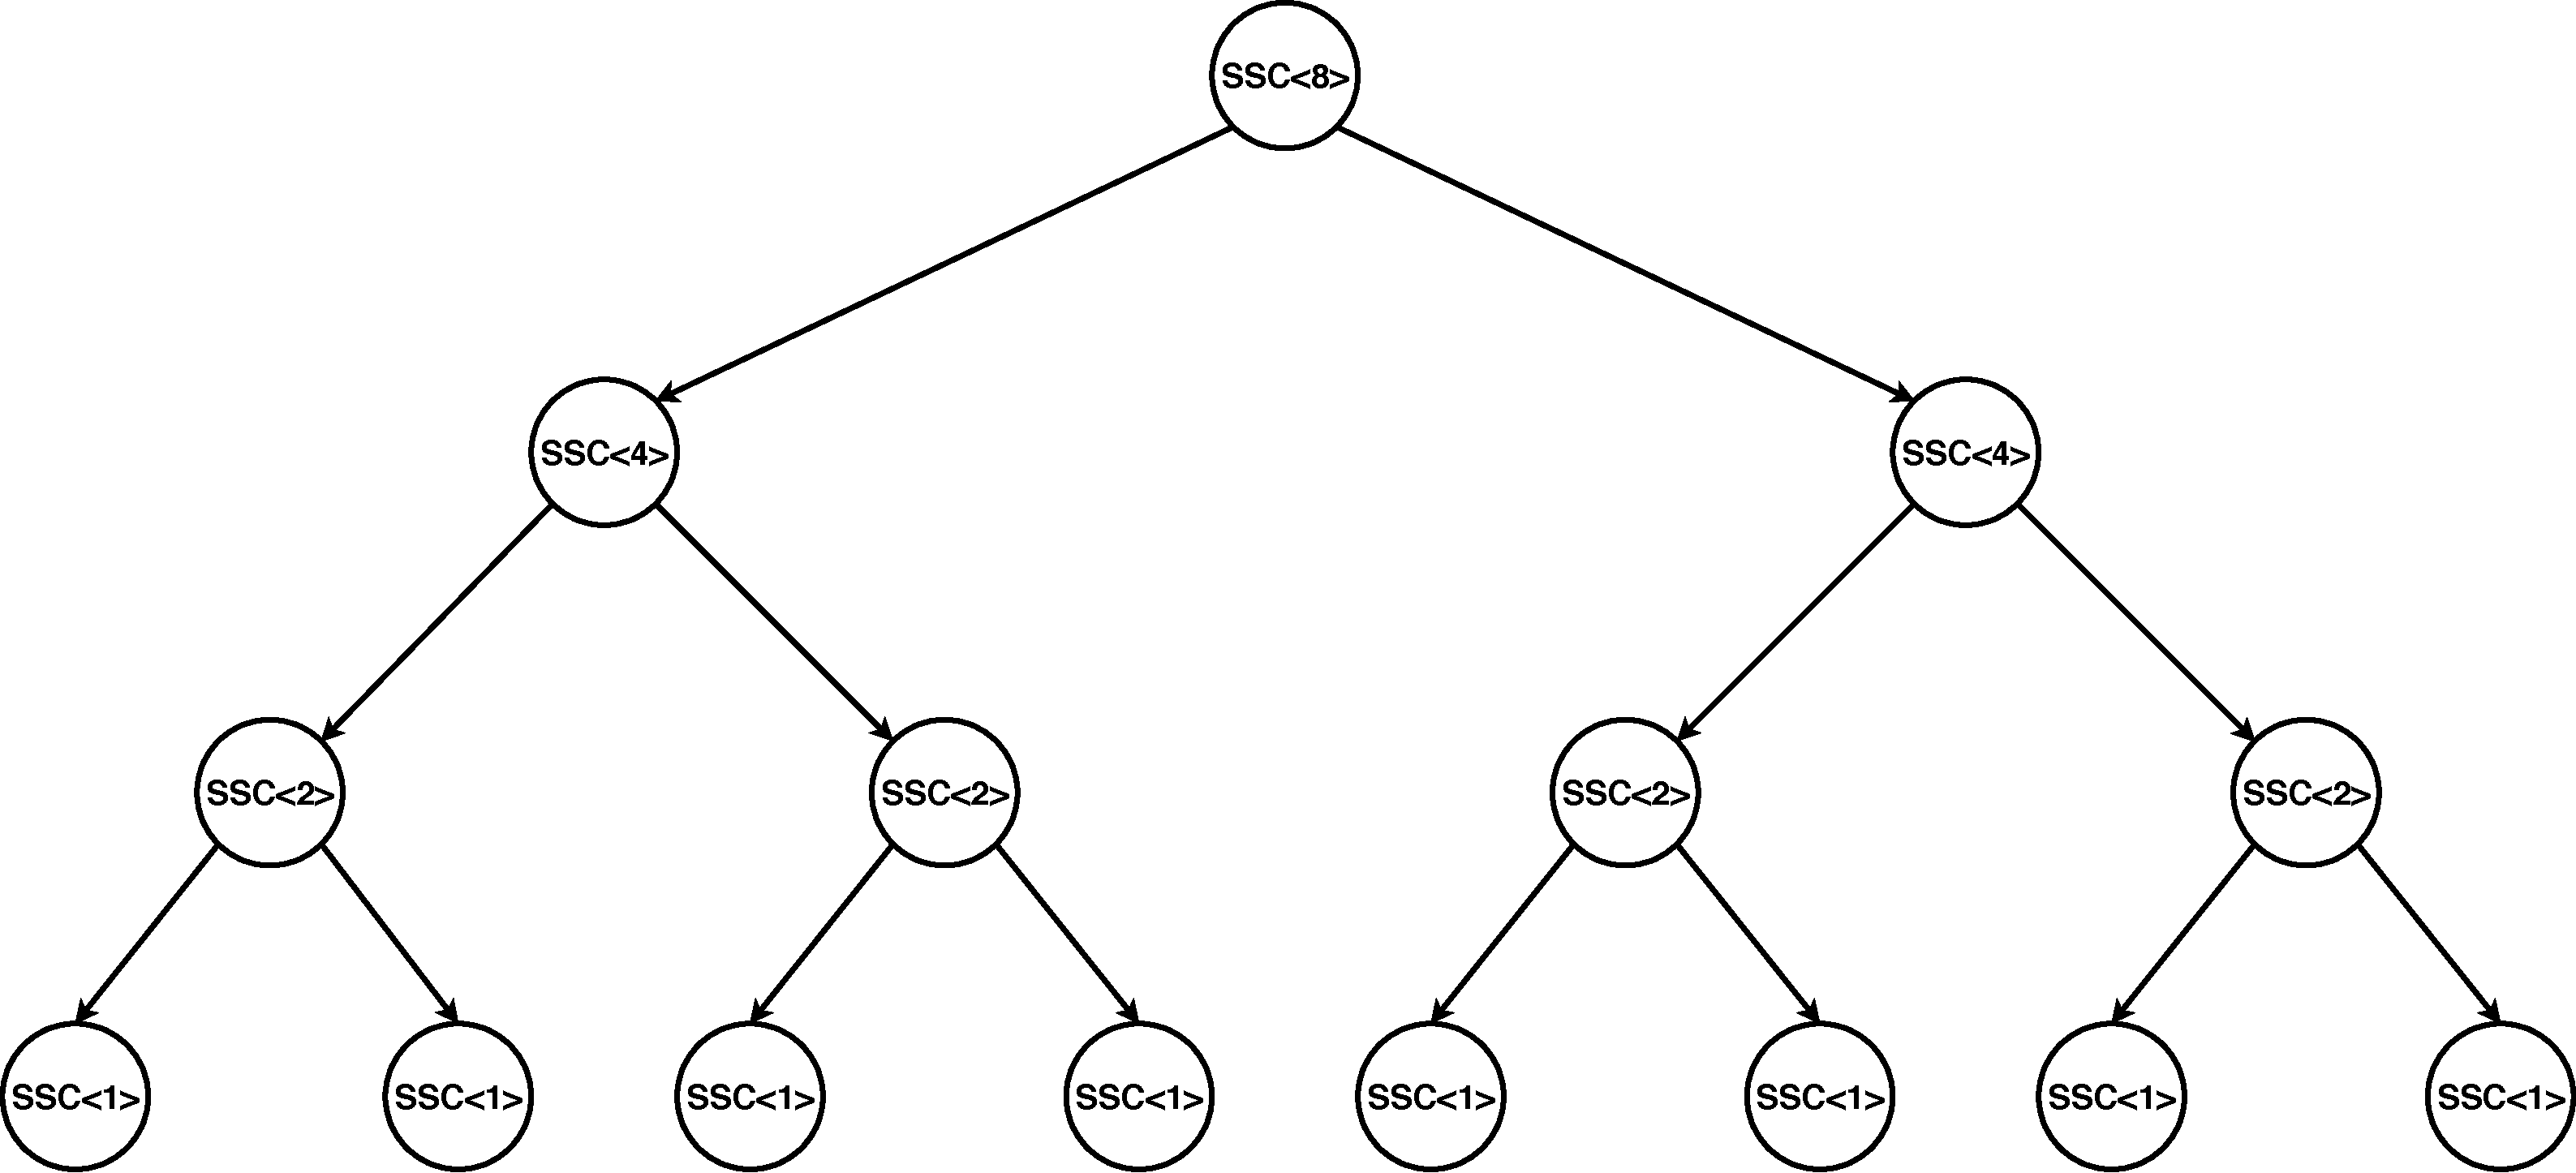
\includegraphics[width=1\textwidth]{./figures/unrolledDecoder.pdf}
	\caption{Unrolled decoder}
	\label{fig:unrolledDecoder}
\end{figure}

\subsection{Cache prefetching}
Performance bottle necks in the modern processors lies in main memory access. To overcome this problem most of modern processors contain smaller fast memory called cache close to the processor. Addition of caches reduces the number of accesses to main memory. However due to the limited cache size it might happen that the requested data not being present in cache, which results in an event called cache-miss. Copied data from main memory to cache has a huge overhead. Cache miss overhead can be reduced by dealing with less memory allocation, in other words reusing the memory as much as possible. Some of the modern processors provide special non blocking instructions which allow cache line prefetching. If the memory access required is known, prefetching instruction can be issued well in advance by software before accessing memory. These instructions if used efficiently, can hide the memory access latency. In this work, decoder implementation is optimized for AMD EPYC platform, which provides cache prefetching instructions through $ \mathtt{3dnow} $ extensions. Due to regular memory access in polar decoder, prefetching instructions are used whenever possible to hide memory access latency.

\subsection{Decoder tree pruning}
Decoding latency can be further reduced by minimizing the number of nodes to be traversed in a decoder tree. This is achieved by pruning decoding tree intelligently at a particular level based on the given SNR and code rate. The level of pruning for a particular SNR and code can be determined through simulations. This information is included in the implementation to determine the pruning level during decoding. Here decoder tree is pruned irrespective frozen pattern type. Main idea is to adoptively prune the decoding tree depending on the SNR and code rate in hand. Tree pruning level is determined before decoder starts, as decoding proceeds and reaches a particular level, frozen pattern is checked whether it matches any special patterns such as R0, R1, RPC or SPC. If it matches any of these patterns then decoding is performed accordingly otherwise further traversing the tree is avoided by decoding through threshold detection and then applying polar transform. This is equivalent to performing a hard decision decoding at that node. two levels of pruning are investigated in this work namely 8 and 4. Pruning level is decided based on SNR and code rate.

Pruning at level 8 reduces the decoding latency from 5.3us to 4.0us and pruning at level 4 reduces latency to 5us from 5.3us (average values). Pruning comes at the expense of error correction performance. However for the scenarios where code rate is low and SNR is good, decoder tree can be safely pruned without losing significant error correction. performance.

%\TODO{Further continuation of this section requires simulation results, estimating the level of pruning depending on SNR and code rate}

\begin{figure}[]
	\centering
	\includegraphics[width=1\textwidth]{./figures/prunedDecoderTree.pdf}
	\caption{Pruned decoder tree}
	\label{fig:prunedDecoderTree}
\end{figure}

%\begin{figure}[]
%	\centering
%	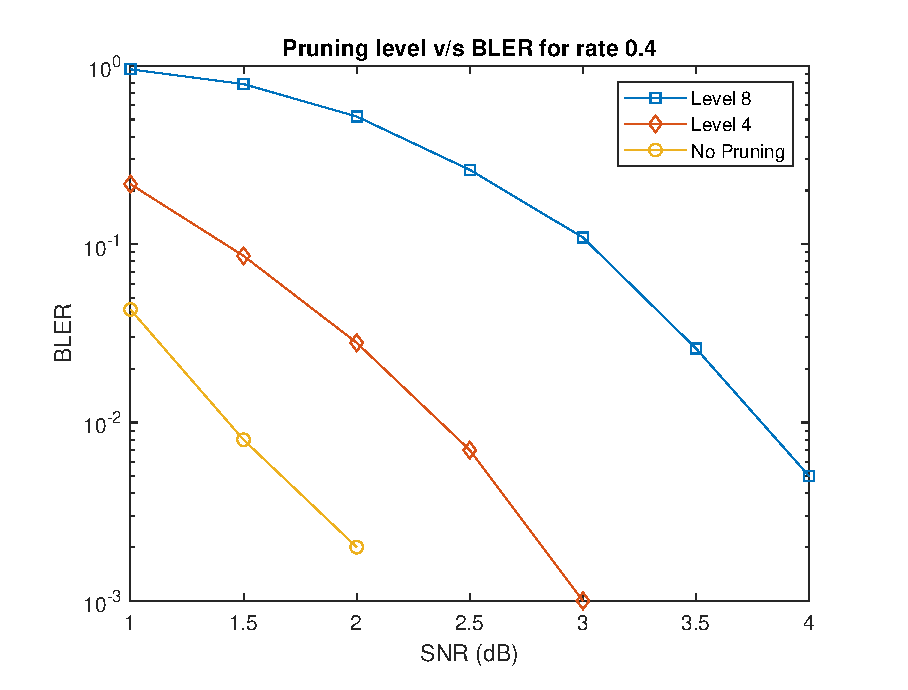
\includegraphics[width=0.7\textwidth]{./figures/rateCurves4.eps}
%	\caption{Pruned code error correction performance}
%	\label{fig:pruningLevelVsRate4}
%\end{figure}
%
%\begin{figure}[]
%	\centering
%	\includegraphics[width=0.7\textwidth]{./figures/rateCurves5.eps}
%	\caption{Pruned code error correction performance}
%	\label{fig:pruningLevelVsRate5}
%\end{figure}

\subsection{Decoding latency comparison}
Following tables represent decoding latency representations
\begin{table}[!h]
	\begin{center}
		\caption{Latency comparison: Plain versus Optimized implementation}
		\label{tab:decoderLatency}
		\begin{tabular}{c|c|c} % <-- Alignments: 1st column left, 2nd middle and 3rd right, with vertical lines in between
			\textbf{ } & Functional & Optimized \\
			\hline
			Latency ($\mu$s) & $283.4$ & $5.3$\\
		\end{tabular}
	\end{center}
\end{table}

\begin{table}[!h]
		\begin{center}
		\caption{Latency comparison: this work versus state of the art \cite{lowLatencySWPolarDec}}
		\label{tab:decoderLatencyStateofTheART}
		\begin{threeparttable}
		\begin{tabular}{c|c|c} % <-- Alignments: 1st column left, 2nd middle and 3rd right, with vertical lines in between
			\textbf{ } & this work & \cite{lowLatencySWPolarDec}* \\
			\hline
			Latency ($\mu$s) & $5.3$ & $8$\\
			\hline
		\end{tabular}
	\begin{tablenotes}\footnotesize
		\item[*] Scaled according to frequency
	\end{tablenotes}
	\end{threeparttable}
	\end{center}
\end{table}

\section{Extract parity check bits}
Parity bits are useful for early termination when decoding performed through list algorithm otherwise they are not required. Polar decoder output is the transmitted codeword of mother code with a block-length $N$ including frozen, information bits and parity check bits. As specified in the 5G standard \cite{3gpp.38.212} for PUCCH three parity bits are calculated ($n_{PC} = 3$) two of these bits are placed in the two least reliable positions out of $K+n_{PC}$, $K+n_{PC}$ positions are most reliable out of $N$. Remaining one parity bit ($ n_{PC}^{wm} = 1 $) is placed in position which corresponds minimum hamming weight row of the polar code generator matrix. This position needs to be identified dynamically since it varies for different code rates. Identifying a minimum hamming weight row requires information about number of ones in each row of generator matrix. One way to know is by storing hamming weight of every row in a look up table and read the values of particular rows. Another way is to exploit the unique structure of the polar generator matrix, i.e number set bits in an integer representing the row index gives hamming weight of a particular row. For the latter method lookup table is not required. In the FEC chain implementation former method is implemented and it has following advantages over latter.

\begin{itemize}  
	\item Modern processors provide instructions to efficiently calculate the number of set bits in an integer. AMD EPYC platform provides $\mathtt{popcnt}$ instruction \cite{AgnerFog}.
	\item Dynamically calculating reduces the number of irregular memory accesses which are required for reading from lookup table hence reducing the cache misses.
\end{itemize}

After extracting parity bits those positions are marked as frozen to ease the extraction of information bits.

\section{Extract Info Bits}
After extracting parity bits codeword of mother code with a block-length $N$ contains frozen and information bits. To obtain only information bits, again at the receiver highest reliability indices must be identified for the same parameters $E$, $K$ and $N$. Same algorithm presented in the encoding chain chapter is used for identifying reliability indices, information bits are read from $K$ most reliable positions out of $N$. There are two ways to extract information bits, One is to take most reliable positions sort them, extract information bits in the order of increasing reliability. Another method is using the previously created frozen pattern, read bits from the location where it contains zero (means that position has information bit). After extensive profiling its identified that sorting is more expensive than going through all $N$ values and reading information bits from non frozen locations. So latter method is included in the FEC chain.

\section{CRC calculation}
For PUCCH and PUSCH, 5G standard specifies different CRC sizes depending on the number of information bits($A$). As specified in \cite{3gpp.38.212} if $ A \ge 20$ $ CRC11 $  otherwise $ CRC6 $ is calculated.  For CRC calculation same algorithm which was used for $ CRC24 $ calculation in PDCCH/PBCH used \cite{Sarwate:1988:CCR:63030.63037}. It is adopted to calculate CRC blockwise for the blocks of size 8-bits with the help of prebuilt lookup tables of $ CRC11 $ and $ CRC6 $. Unlike PDCCH/PBCH CRC calculation, this is a generic implementation, in other words type of CRC is decided at runtime based on the value of $A$ and gets calculated with same generic logic.

\section{Decoding FEC chain latency results}

$I_{IL} = 0, n_{max} = 10, n_{pc} = 3 ,n_{pc}^{wm} = 1, I_{BIL} = 1, E = 1692, K = 512$.
\begin{table}[!h]
	\begin{center}
		\caption{Latency comparison: Polar decoding FEC chain}
		\label{tab:decodingFECChainLatency}
		\begin{tabular}{c|c|c} % <-- Alignments: 1st column left, 2nd middle and 3rd right, with vertical lines in between
			\textbf{ } & Functional & Optimized \\
			\hline
			Latency ($\mu$s) & $346.4$ & $30$\\
		\end{tabular}
	\end{center}
\end{table}
          % Include ... / Einbinden des Kapitels ...
        \chapter{Conclusion and Outlook} \label{chap:conclusion}
The objective of this work is to study the feasibility of developing polar FEC chain of 5G in software on general-purpose-processor while satisfying stringent latency requirements. In other words, all the components of encoder and decoder FEC chain are developed on general purpose AMD EPYC processor. The software satisfies latency constraint of less than 50$\mu$s. In the first part of the thesis, we provide necessary background about polar encoding/decoding and computer architecture. In the second part, we develop encoding and decoding FEC chains and optimize them to satisfy the necessary latency constraints. \newline

To begin with, we provided necessary mathematical background about polar code construction, polar encoding, and decoding. Including different polar decoding algorithms. To understand FEC chain development in software it is necessary to know the basics of modern computer architecture. Computer architecture section talks about pipelining, cache memory and vector processing units in modern general purpose processors. \newline

In the next chapter, we talk about the details of polar encoding FEC chain. In this chapter, we analyze the different components of the FEC chain to identify latency contributors. Each of these latency contributors is further studied to reformulate the algorithm to avoid costly operations. Algorithms are reformulated to fit into specialized functional units of modern processors such as vector processing units. Vector processing units allow data parallelism in addition to supporting very fast mathematical computations. The encoding,  major latency contributors were polar code construction, CRC calculation, encoding, and rate matching. A wide range of optimization techniques is employed to reduce the latency both algorithmic and platform specific. Namely, reducing algorithm complexity, using lookup tables, compiler hints for better instruction scheduling, vector processing instructions for data parallelism and avoiding superfluous copy operations et cetera. Optimizations reduced the worst-case latency of the encoding FEC chain from $451 \mu$s to $40\mu$s which is more than 10x reduction in latency. \newline

For the decoding FEC chain again same steps as encoding chain are followed to identify the latency contributors. Major contributors in decoding FEC chain were channel deinterleaver, subblock deinterlever, polar decoder, parity bit extractor, and CRC calculation. Decoding FEC chain extensively uses SIMD, bit count, cache prefetching instructions to reduce latency. Subblock deinterleaving operation is divided into three primitive small operations which are implemented efficiently with $\mathtt{permute}$ and $\mathtt{blend}$ vector instructions. The polar decoder is optimized by implementing XOR, CN, VN, bit combination and frozen pattern identification operations using vector processing instructions. Parity bit extractor optimized by avoiding expensive remove and erase operations instead uses modified algorithm marking indexes and dynamically calculating hamming weights of generator matrix rows. Finally, for CRC calculation an algorithm based on lookup table is developed based on \cite{Sarwate:1988:CCR:63030.63037} which processes block of data bits to calculate CRC. These optimizations significantly reduced the latency of decoding FEC chain from $391 \mu$s to $40\mu$s almost a 10x reduction in latency. \newline

As an outlook, for the above stated decoding FEC chain, decoder is developed with \emph{fast-SSC} algorithm. This algorithm has much lower error correction performance than similar block-length LDPC and Turbo counterparts. As part of this work, \emph{CRC-Aided Successive Cancellation List} (\emph{CA-SCL})\cite{SCL} decoding algorithm is also implemented, however, it is not optimized for software. \emph{CA-SCL} ideally suits very low SNR scenarios such as mmWave communication. It has approximately $1.5dB$ gain over \emph{fast-SSC} algorithm for $N=2048$ and list size $L = 8$. Ideal continuation of this work would be to extend the decoding chain by incorporating \emph{CA-SCL} algorithm to the FEC chain. It would be interesting to see the latency values of this algorithm, which has expensive \emph{sort} and \emph{copying} operations.   % Include conclusion/summary / Einbinden des Kapitels Zusammenfassung/Ausblick
        
        \cleardoubleemptypage

% ########################################
% Appendix / Anhang:
% ########################################

% roman page numbering, starting with page number 1 (capitals)/ roemische Seitennummerierung beginnend mit Seite 1 (gross)
    \appendix
    \setcounter{page}{1}
    \pagenumbering{Roman}

        % Use IEEE DIN 1505 style for bibliography / Literaturverzeichnisses
        \bibliographystyle{IEEEtr}
        \nocite{*}              % Include all references without checking / Alle References immer aufführen
        \bibliography{literature}

\end{document}

%
% EOF!
%